\subsection{Definition of vector bundles}

7.1.1. A vector chart of M is a triple \(t = (U, \varphi, F)\) , where U is an open subset of B, F is a Banach space, and \(\varphi\) is a bijection from \(\pi^{-1}(U)\) onto \(U \times F\) such that \(\pi(\varphi^{-1}(b, h)) = b\) for all \(b \in B\) and all \(h \in F\) . We say that U is the domain of the vector chart \(t\) and that \(t\) is a vector chart of M at \(b \in B\) if \(b \in U\) . For every \(b \in U\) , one denotes by \(t_b\) the bijection from F to \(M_b\) defined by \(t_b(h) = \varphi^{-1}(b, h)\) for \(h \in F\) .

7.1.2. Two vector charts \(t = (\mathrm{U}, \varphi, \mathrm{F})\) and \(t' = (\mathrm{U}', \varphi', \mathrm{F}')\) of \(\mathbf{M}\) are \(\mathbf{C}'\) -compatible (or simply compatible) if there exists a map \(\lambda\) of class \(\mathbf{C}'\) from the manifold \(\mathrm{U} \cap \mathrm{U}'\) into the Banach space \(\mathcal{L}(\mathrm{F}; \mathrm{F}')\) such that:

\[
t _ {b} = t _ {b} ^ {\prime} \circ \lambda (b) \quad \text { for all } b \in \mathbf {U} \cap \mathbf {U} ^ {\prime}.
\]

7.1.3. A set of vector charts of M is said to be a C'-vector atlas (or simply vector atlas) of M if it consists of pairwise C'-compatible vector charts whose domains have union B. Two vector atlases A and B of M are said to be C'-equivalent (or equivalent) if A ∪ B is again a vector atlas of M. This relation is an equivalence relation.

7.1.4. A vector bundle structure of class \(C^{r}\) (basis B) on M is the data of a class of equivalent vector atlases (Sets, Chap. II, § 6, no. 9). A vector chart belonging to a vector atlas of this class is called a vector chart of the vector bundle M.

Let M be a vector bundle with base B. For every \(b \in B\) there exists on the fiber \(M_{b}\) a Banach space structure, and only one such that, for every vector chart \(t = (\mathbf{U}, \varphi, \mathbf{F})\) of the vector bundle M at b, the map \(t_{b}\) is an isomorphism from F onto \(M_{b}\) .

Let \(c = (\mathbf{U}, \psi, \mathbf{E})\) be a chart of the manifold \(\mathbf{B}\) and let \(t = (\mathbf{U}, \varphi, \mathbf{F})\) be a vector chart of the vector bundle \(\mathbf{M}\) , with the same domain \(\mathbf{U}\) . For \(x \in \pi^{-1}(\mathbf{U})\) , set:

\[
\alpha (x) = (\psi (\pi (x)), t _ {\pi (x)} ^ {- 1} (x)).
\]

Then, the triple \((\pi^{-1}(\mathbf{U}), \alpha, \mathbf{E} \times \mathbf{F})\) is a chart of the set M. There exists on M a manifold structure of class \(C^{r}\) and only one (called the underlying structure of M) for which all the charts thus obtained are charts of the manifold M. The triple \((\mathbf{M}, \mathbf{B}, \pi)\) is then a fibration (6.1.1).

7.1.5. Let F be a Banach space. Set \(M = B \times F\) , the map being the first projection. There exists on M a vector bundle structure (with base B), and only one, for which \((\mathbf{B}, \mathbf{Id}_{\mathbf{M}}, \mathbf{F})\) is a vector chart. We say that \(B \times F\) endowed with this structure is the trivial vector bundle over the base B with fiber F, and it is sometimes denoted by \(F_{B}\) . The manifold structure of \(F_{B}\) is the product manifold structure, and for every \(b \in B\) , the map \(h \mapsto (b, h)\) is a Banach space isomorphism from F onto the fiber of \(F_{B}\) at the point \(b \in B\) . One often denotes by 0 a trivial vector bundle whose fiber is reduced to 0.

7.1.6. Let M be a vector bundle with base B. For \(b \in B\) we call the dimension (finite or \(+\infty\) ) of the Banach space \(M_{b}\) the rank of M at b, and denote it by \(\operatorname{rg}_{b}(\mathbf{M})\) . One has \(\dim_{x}\mathbf{M} = \dim_{b}\mathbf{B} + \operatorname{rg}_{b}\mathbf{M}\) for \(b = \pi(x)\) . The function \(b \mapsto \operatorname{rg}_{b}\mathbf{M}\) is locally constant. We say that M is of finite rank if \(\operatorname{rg}_{b}\mathbf{M} < +\infty\) for all \(b \in B\) .

\subsection{Morphisms of vector bundles}

7.2.1. Let B and B' be two manifolds and let f be a morphism from B to B'. Let M be a vector bundle with base B and M' a vector bundle with base B'. We say that a map g from M to M' is an f-morphism of vector bundles if the following condition is satisfied:

For every point \(b_0 \in \mathbf{B}\) , there exists a vector chart \(t = (\mathrm{U}, \varphi, \mathrm{F})\) of \(\mathbf{M}\) at \(b_0\) , a vector chart \(t' = (\mathrm{U}', \varphi', \mathrm{F}')\) of \(\mathbf{M}'\) at \(f(b_0)\) and a mapping \(\lambda\) of class \(\mathbf{C}'\) from \(\mathbf{U}\) into \(\mathcal{L}(\mathbf{F}; \mathbf{F}')\) such that \(f(\mathbf{U}) \subset \mathbf{U}'\) and that \(g_b \circ t_b = t_{f(b)}' \circ \lambda(b)\) for all \(b \in \mathbf{U}\) , where \(g_b\) is the restriction of \(g\) to \(\mathbf{M}_b\) .

Under these hypotheses, \(g\) is a morphism of manifolds and for every \(b \in B\) , \(g\) induces a continuous linear map from \(M_b\) to \(M_{f(b)}'\) . We call the rank (finite or \(+\infty\) ) of the linear map \(g_b\) the vector rank of \(g\) at \(b \in B\) , and denote it by \(\text{rg}_b(g)\) .

Conversely, if \(r \geqslant \infty\) or if \(M\) is of finite rank, an \(f\)-morphism of fibrations from \((M, B, \pi)\) to \((M', B', \pi')\) which induces on each fiber \(M_b\) a linear map from \(M_b\) to \(M_{f(b)}'\) (for every \(b \in B\) ), is an \(f\)-morphism of vector bundles.

7.2.2. Let moreover \(f'\) be a morphism of \(B'\) into a manifold \(B''\) . If \(g\) is an \(f\)-morphism of \(M\) to \(M'\) and if \(g'\) is an \(f'\)-morphism of \(M'\) into a vector bundle \(M''\) with base \(B''\) , the map \(g' \circ g\) is an \((f' \circ f)\)-morphism of \(M\) to \(M''\) . One has \((g' \circ g)_b = g_{f(b)}' \circ g_b\) for all \(b\) in \(B\) .

7.2.3. Let M and M' be two vector bundles with the same base B. One calls a B-morphism, or simply a morphism from M to M', any \(\mathrm{Id}_{\mathbf{B}}\)-morphism. The composite of two morphisms is a morphism.

Let \(g\) be a morphism of vector bundles from \(M\) to \(M'\) ; if \(g\) is bijective, it is an isomorphism of the manifold \(M\) onto the manifold \(M'\) , the inverse mapping \(g^{-1}\) is a morphism of vector bundles from \(M'\) to \(M\) and one has \((g^{-1})_b = g_b^{-1}\) for all \(b\) in \(B\) . The map \(g\) is then an isomorphism of vector bundles.

7.2.4. Let \(f\) be a morphism of a manifold \(\mathbf{B}'\) to \(\mathbf{B}\) and let \(\mathbf{M}\) be a vector bundle with base \(\mathbf{B}\) . Set \(\mathbf{M}' = \mathbf{B}' \times_{\mathbf{B}} \mathbf{M}\) and denote by \(\pi'\) (resp. \(g\) ) the restriction to \(\mathbf{M}'\) of the projection of \(\mathbf{B}' \times \mathbf{M}\) onto \(\mathbf{B}'\) (resp. \(\mathbf{M}\) ). On \(\mathbf{M}'\) there exists a vector bundle structure with base \(\mathbf{B}'\) (relative to \(\pi'\) ) and only one for which \(g\) is an \(f\)-morphism. One says that \(\mathbf{M}'\) is the vector bundle with base \(\mathbf{B}'\) inverse image of \(\mathbf{M}\) by \(f\) and is denoted \(f^* \mathbf{M}\) ; the \(f\)-morphism \(g\) is called the canonical \(f\)-morphism of \(f^* \mathbf{M}\) to \(\mathbf{M}\) .

The manifold structure of \(f^{*}\mathbf{M}\) is that of the fibered product of the manifolds \(\mathbf{B}'\) and \(\mathbf{M}\) over \(\mathbf{B}\) (5.11.2); for every \(b\in\mathbf{B}'\) , the map \(x\mapsto(b,x)\) is an isomorphism of Banach spaces from \(\mathbf{M}_{f(b)}\) onto \((f^{*}\mathbf{M})_{b}\) .

The formation of inverse images of vector bundles is transitive.

Let N' be a vector bundle with base B' and let h be an f-morphism from N' to M. There exists one and only one B'-morphism \(\tilde{h}\) from N' to \(f^{*}M\) such that \(h = g \circ \tilde{h}\) .

Let N be a vector bundle with base B and let v be a B-morphism from N to M. There exists one and only one B'-morphism, denoted \(f^{*}v\) , from \(f^{*}N\) to \(f^{*}M\) such that the diagram

\pandocbounded{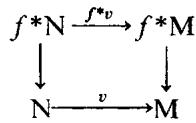
\includegraphics[keepaspectratio]{images/part001_e53c46a7.jpg}}

is commutative.

7.2.5. Let B' be a submanifold of B and let i be the canonical injection from B' into B. If M is a vector bundle with base B, the inverse image \(i^*M\) is called the vector bundle induced on B' by M and is denoted \(M|_{B'}\). If \(t = (\mathrm{U}, \varphi, \mathrm{F})\) is a vector chart of M, then \((\mathrm{U} \cap \mathrm{B}', \varphi | \pi^{-1}(\mathrm{U} \cap \mathrm{B}'), \mathrm{F})\) is a vector chart of \(M|_{B'}\). The canonical f-morphism from \(M|_{B'}\) into M is an isomorphism of manifolds from \(M|_{B'}\) onto the submanifold \(\pi^{-1}(\mathrm{B}')\) of M.

7.2.6. Let \(f\) be a morphism from a manifold B' into B and let M (resp. M') be a vector bundle with base B (resp. B'). One calls an \(f\)-comorphism from M into M' a B'-morphism from \(f^{*}M\) into M'. When B = B' and \(f = \mathrm{Id}_{\mathbf{B}}\) , the data of an f-comorphism from M into M' is equivalent to the data of a B-morphism from M into M'.

Let \(g\) be an \(f\)-comorphism of \(\mathbf{M}\) to \(\mathbf{M}'\) . For every \(b \in \mathbf{B}'\) , the map \(g_b: x \mapsto g(b, x)\) from \(\mathbf{M}_{f(b)}\) to \(\mathbf{M}_b'\) is a continuous linear map.

Additionally, let \(f'\) be a morphism of a manifold \(B''\) to \(B'\) and let \(h\) be an \(f'\)-comorphism of \(M'\) into a vector bundle \(M''\) with base \(B''\) . The map \(h \circ f'^{*}g\) of \(f'^{*}(f^{*}M) = (f \circ f')^{*}M\) to \(M''\) is then an \((f \circ f')\)-comorphism of \(M\) to \(M''\) , denoted \(h \circ g\) . For \(b \in B''\) , one has

\[
(h \circ g) _ {b} = h _ {b} \circ g _ {f ^ {\prime} (b)}.
\]

\subsection{Multilinear morphisms}

7.3.1. Let \(M_{1},\ldots,M_{d}\) and N be vector bundles with base B, and let u be a map from the set \(M_{1}\times_{B}\ldots\times_{B}M_{d}\) into N. One says that u is a multilinear morphism (or d-linear) if the following condition is satisfied:

For every \(b_0 \in \mathbf{B}\) , there exists an open neighborhood \(\mathbf{U}\) of \(b_0\) in \(\mathbf{B}\) , vector charts \(t^j = (\mathbf{U}, \varphi^j, \mathbf{F}^j)\) of \(\mathbf{M}_j\) (for \(1 \leqslant j \leqslant d\) ) and \(t = (\mathbf{U}, \varphi, \mathbf{F})\) of \(\mathbf{N}\) , and a map \(\lambda\) of class \(\mathbf{C}^r\) from \(\mathbf{U}\) into the Banach space \(\mathcal{L}(\mathbf{F}^1, \ldots, \mathbf{F}^d; \mathbf{F})\) of continuous d-linear maps from \(\mathbf{F}^1 \times \cdots \times \mathbf{F}^d\) to \(\mathbf{F}\) , such that:

\[
(t _ {b} \circ \lambda (b)) (x _ {1}, \dots , x _ {d}) = u (t _ {b} ^ {1} (x _ {1}), \dots , t _ {b} ^ {d} (x _ {d}))
\]

for all \(b \in \mathbf{U}\) and all \(x_{j} \in \mathbf{F}^{j}\) .

Every multilinear morphism \(u\) is a morphism of manifolds from the fibered product \(\mathbf{M}_{1} \times_{\mathbf{B}} \cdots \times_{\mathbf{B}} \mathbf{M}_{d}\) to \(\mathbf{N}\) and induces for every \(b \in \mathbf{B}\) a continuous \(d\)-linear map \(u_b\) from \((\mathbf{M}_{1})_{b} \times \cdots \times (\mathbf{M}_{d})_{b}\) to \(\mathbf{N}_{b}\) .

If \(f\) is a morphism from B into a manifold \(\mathbf{B}'\) , a multilinear morphism from \(\mathbf{M}_1 \times_{\mathbf{B}} \cdots \times_{\mathbf{B}} \mathbf{M}_d\) into a vector bundle \(\mathbf{M}'\) with base \(\mathbf{B}'\) is by definition the composite of a multilinear morphism from \(\mathbf{M}_1 \times_{\mathbf{B}} \cdots \times_{\mathbf{B}} \mathbf{M}_d\) to \(f^*\mathbf{M}'\) with the canonical \(f\)-morphism of \(f^*\mathbf{M}'\) to \(\mathbf{M}'\) .

A bilinear morphism is also called a pairing. For \(d=1\) , a linear morphism is a morphism in the sense of 7.2.1. For \(d=0\) , a 0-linear morphism is identified with a section of N (7.4).

7.3.2. An algebra bundle over base B is a vector bundle A over base B, equipped with a pairing of \(A \times_{B} A\) into A. Each fiber \(A_{b}\) is then equipped with a K-algebra structure. If for every \(b \in B\) the algebra \(A_{b}\) has an identity element, denoted \(e_{b}\) , the map \(b \mapsto e_{b}\) is a section of A (cf. 7.4). An algebra bundle A is said to be locally trivial if, for every point \(b_{0}\) of B, there exists a vector chart \(t = (\mathrm{U}, \varphi, \mathrm{E})\) from A at the point \(b_{0}\) and a K-algebra structure on E such that \(t_{b}\) is an isomorphism of algebras from E onto \(A_{b}\) for all \(b \in U\) .

7.3.3. Let A be a bundle of associative algebras with unit element over base B. One calls a bundle of A-modules over base B a vector bundle M over base B equipped with a pairing \(m: A \times_{B} M \to M\) such that the map \(m_{b}: A_{b} \times M_{b} \to M_{b}\) defines, for all \(b \in B\) , a structure of \(A_{b}\)-module on the fiber \(M_{b}\) .

Let M and M′ be two vector bundles in A-modules. We call an A-homomorphism from M to M′ any morphism \(g: M \rightarrow M'\) of vector bundles over the base B which induces for every b in B an \(A_b\)-linear map from \(M_b\) to \(M_b'\) .

Suppose A is locally trivial. We say that a bundle M of A-modules is locally trivial if for every point \(b_0\) of B, there exists a vector chart \(t = (U, \varphi, E)\) from A at \(b_0\) as in 7.3.2, a vector chart \(t' = (U, \varphi', L)\) from M at \(b_0\) , and a structure of E-module on L such that, for every \(b \in U\) , \(t_b'\) is a \(t_b\)-isomorphism of the \(A_b\)-module \(M_b\) onto the E-module L.

7.3.4. Let A be a Banach algebra over K (for example, a field equipped with a finite-dimensional K-algebra structure). The trivial bundle \(A_{B}\) is then a locally trivial algebra bundle. A locally trivial bundle M in \(A_{B}\)-modules is also called a vector bundle over A (with base B). The fibers \(M_{b}\) are then topological A-modules. An f-morphism u from M to another vector bundle over A is said to be A-linear if the maps \(u_{b}\) are A-linear for all \(b \in B\) .

\subsection{Sections}

7.4.1. Let M be a vector bundle with base B. For every open set U of B, we denote by \(\mathcal{S}_{\mathbf{M}}^{r}(\mathbf{U})\) the set of sections of class \(C^r\) of M over U, that is, morphisms \(s\) of class \(C^r\) from U into M such that \(s(b) \in M_b\) for all \(b \in \mathbf{U}\) . This set is equipped with a module structure over the ring \(\mathcal{C}^r(\mathbf{U})\) of morphic functions by the rules:

\begin{enumerate}
\def\labelenumi{(\arabic{enumi})}
\tightlist
\item
\end{enumerate}

\[
(s + s ^ {\prime}) (b) = s (b) + s ^ {\prime} (b)\tag{2}
\]

\[
(\varphi . s) (b) = \varphi (b). s (b)
\]

for \(s, s'\) in \(\mathcal{S}_{\mathrm{M}}^{r}(\mathrm{U})\) and \(\varphi\) in \(\mathcal{C}^{r}(\mathrm{U})\) . When the open set U varies, one obtains a sheaf \(\mathcal{S}_{\mathrm{M}}^{r}\) of maps from B into M (cf. no. 5.4.1), called the sheaf of sections of M.

7.4.2. Let \(M_{1},\ldots,M_{d}\) and N be vector bundles over the base B, and let u be a multilinear morphism from \(M_{1}\times_{B}\ldots\times_{B}M_{d}\) into N. For \(1\leqslant j\leqslant d\) let us give a section \(s_{j}\) of \(M_{j}\) on an open set U of B; one defines a section \(u(s_{1},\ldots,s_{d})\) of N on U by the formula:

\[
u (s _ {1}, \dots , s _ {d}) (b) = u _ {b} (s _ {1} (b), \dots , s _ {d} (b)) \quad \text {   for   } b \in \mathrm{U}.
\]

The map \((s_1, \ldots, s_d) \mapsto u(s_1, \ldots, s_d)\) is \(\mathcal{C}^r(\mathrm{U})\) -multilinear. It is sometimes denoted \(\mathcal{S}(u)\) .

7.4.3. Let \(f\) be a morphism of a manifold \(\mathbf{B}'\) to \(\mathbf{B}\) and let \(\mathbf{M}\) be a vector bundle with base \(\mathbf{B}\) . For every open set \(\mathbf{U}\) of \(\mathbf{B}\) and every \(s \in \mathcal{S}_{\mathbf{M}}^{r}(\mathbf{U})\) , the map \(x \mapsto (x, s(f(x)))\) is a section of class \(\mathbf{C}^r\) of \(f^{*}\mathbf{M}\) on the open subset \(f^{-1}(\mathbf{U})\) , denoted \(f^{*}s\) and called the inverse image of \(s\) by \(f\) . The map \(s \mapsto f^{*}s\) from \(\mathcal{S}_{\mathbf{M}}^{r}(\mathbf{U})\) to \(\mathcal{S}_{f^{*}\mathbf{M}}^{r}(f^{-1}(\mathbf{U}))\) is semilinear with respect to the homomorphism \(g \mapsto g \circ (f|f^{-1}(\mathbf{U}))\) from \(\mathcal{C}^{r}(\mathbf{U})\) to \(\mathcal{C}^{r}(f^{-1}(\mathbf{U}))\) .

If moreover N is a vector bundle over B' and g is an f-comorphism from M to N, one sometimes writes \(\mathcal{S}(g)\) for the map \(s \mapsto g \circ f^{*}s\) from \(\mathcal{S}_{\mathbf{M}}^{\mathbf{r}}(\mathbf{U})\) to \(\mathcal{S}_{\mathbf{N}}^{\mathbf{r}}(f^{-1}(\mathbf{U}))\) .

7.4.4. Let M be a vector bundle over the base B, of finite rank. A frame of M over an open set U of B is called a finite sequence \((s_{1},\ldots,s_{n})\) of sections of M over U such that \((s_{1}(b),\ldots,s_{n}(b))\) is a basis of the vector space \(M_{b}\) for all \(b\in U\) . The sequence \((s_{1},\ldots,s_{n})\) is then a basis of the \(\mathcal{C}^{r}(\mathrm{U})\)-module \(\mathcal{S}_{\mathbf{M}}^{r}(\mathrm{U})\) . If f is a morphism from a manifold \(B'\) into B, the sections \(f^{*}s_{j}\) form a frame of \(f^{*}\mathbf{M}\) on \(f^{-1}(\mathbf{U})\) .

7.4.5. Let L be a field, equipped with a structure of finite-dimensional K-algebra, and let (M, B, π) be a fibration. Suppose given on each fiber \(M_{b}\) a vector space structure over L, of finite dimension. There then exists at most one vector bundle structure on M with base B, compatible with the map π, the manifold structure of M, and the L-vector structures on the fibers (7.3.4). For one to exist, it is necessary and sufficient that the following condition be satisfied:

(FV) For every \(b_0 \in \mathbf{B}\) , there exists an open neighborhood \(\mathbf{U}\) of \(b_0\) in \(\mathbf{B}\) and an isomorphism of manifolds \(\varphi\) from \(\pi^{-1}(\mathbf{U})\) onto the product \(\mathbf{U} \times \mathbf{F}\) of \(\mathbf{U}\) by a vector space \(\mathbf{F}\) over \(\mathbf{L}\) of finite dimension, such that for every \(b \in \mathbf{U}\) the bijection \(\varphi_b\) from \(\mathbf{M}_b\) onto \(\mathbf{F}\) induced by \(\varphi\) is an isomorphism of vector spaces over the field \(\mathbf{L}\) .

The triples (U, \(\varphi\) , F) satisfying (FV) are then vector charts of the vector bundle M.

Condition (FV) is equivalent to:

(FV') For every \(b_0 \in \mathbf{B}\) there exists an integer \(n\) and \(n\) sections \(s_1, \ldots, s_n\) of \(\mathbf{M}\) on an open neighborhood \(\mathbf{U}\) of \(b_0\) such that the map

\[
(b, a _ {1}, \dots , a _ {n}) \mapsto a _ {1} s _ {1} (b) + \dots + a _ {n} s _ {n} (b)
\]

is an isomorphism from the manifold \(\mathbf{U} \times \mathbf{L}^{n}\) to the manifold \(\pi^{-1}(\mathbf{U})\) .

7.4.6. Let \(M_{1},\ldots,M_{d}\) and N be vector bundles with base B, the \(M_{j}\) being of finite rank. Suppose that for every open set U of B a \(\mathcal{C}^{r}(\mathrm{U})\)-multilinear map \(\varphi_{\mathrm{U}}\) from \(\mathcal{S}_{\mathrm{M}_{1}}^{\mathrm{r}}(\mathrm{U})\times\cdots\times\mathcal{S}_{\mathrm{M}_{d}}^{\mathrm{r}}(\mathrm{U})\) to \(\mathcal{S}_{\mathrm{N}}^{\mathrm{r}}(\mathrm{U})\) is given, such that for \(V \subset U\) one has:

\[
\varphi_ {\mathrm{U}} (s _ {1}, \dots , s _ {d}) | \mathrm{V} = \varphi_ {\mathrm{V}} (s _ {1} | \mathrm{V}, \dots , s _ {d} | \mathrm{V}).
\]

There then exists a multilinear morphism \(u\) of \(\mathbf{M}_1 \times_{\mathbf{B}} \ldots \times_{\mathbf{B}} \mathbf{M}_d\) to \(\mathbf{N}\) such that \(\varphi_{\mathbf{U}}(s_1, \ldots, s_d) = u(s_1, \ldots, s_d)\) for any sections \(s_j\) of \(\mathbf{M}_j\) on the open subset \(\mathbf{U}\) of \(\mathbf{B}\) .

7.4.7. Let \(f\) be a morphism of a manifold \(\mathbf{B}'\) to \(\mathbf{B}\) and let \(\mathbf{M}\) (resp. \(\mathbf{M}'\) ) be a vector bundle with base \(\mathbf{B}\) (resp. \(\mathbf{B}'\) ) and of finite rank. Suppose that for every open set \(\mathbf{U}\) of \(\mathbf{B}\) a continuous \(\mathcal{C}^{r}(\mathbf{U})\)-semilinear map \(\varphi_{\mathbf{U}}\) from \(\mathcal{S}_{\mathbf{M}}^{r}(\mathbf{U})\) to \(\mathcal{S}_{\mathbf{M}'}^{r}(f^{-1}(\mathbf{U}))\) is given, such that

\[
\varphi_ {\mathbf {U}} (s) | f ^ {- 1} (\mathbf {V}) = \varphi_ {\mathbf {V}} (s | \mathbf {V})
\]

for every open set \(V \subset U\) . There then exists a unique f-comorphism g from M to \(M'\) such that \(\varphi_{\mathrm{U}}(s) = \mathcal{S}(g)(s)\) for all \(s \in \mathcal{S}_{\mathrm{M}}^{r}(\mathrm{U})\) .

*7.4.8. Let \(\mathcal{F}\) be a sheaf of modules over the sheaf of rings \(\mathcal{C}_{\mathrm{B}}^{r}\) . We say that \(\mathcal{F}\) is locally free if for every \(b \in \mathrm{B}\) there exists an open neighborhood U of \(b\) and an integer \(n\) such that \(\mathcal{F}|\mathrm{U}\) is isomorphic (as a sheaf of \(\mathcal{C}_{\mathrm{U}}^{r}\) -modules) to the sheaf \((\mathcal{C}_{\mathrm{U}}^{r})^{n}\) .

If M is a vector bundle over the base B of finite rank, the sheaf \(\mathcal{S}_{\mathrm{M}}^{r}\) is locally free. Conversely, for every locally free sheaf \(\mathcal{F}\) on B, there exists a vector bundle M and an isomorphism of sheaves of \(\mathcal{S}_{\mathrm{M}}^{r}\) onto \(\mathcal{F}\) . If M' is another finite-rank vector bundle with base B, the map \(g \mapsto \mathcal{S}(g)\) is a bijection from the set of B-morphisms from M to M' onto the set of sheaf morphisms of \(\mathcal{C}^{r}\)-modules from \(\mathcal{S}_{\mathrm{M}}^{r}\) to \(\mathcal{S}_{\mathrm{M}'}^{r}\) .

\subsection{Vector subbundles, quotient vector bundles, exact sequences}

In this number, we call a vector bundle a vector bundle with base B and a morphism of vector bundles an \(\mathrm{Id}_{\mathbf{B}}\)-morphism.

7.5.1. Let M be a vector bundle. A subset M' of M is called a vector subbundle of M if, for every point \(b \in B\) , there exists a vector chart \(t = (\mathbf{U}, \varphi, \mathbf{E})\) from M at b and a closed vector subspace F of E admitting a topological complement, such that

\[
\varphi (\pi^ {- 1} (\mathrm{U}) \cap \mathrm{M} ^ {\prime}) = \mathrm{U} \times \mathrm{F}.
\]

Under these conditions, there exists on M′ a vector bundle structure, and only one, for which the canonical injection of M′ into M is a morphism. For each \(b \in B\) , the fiber \(M_{b}'\) of M' is the closed vector subspace \(M' \cap M_{b}\) of \(M_{b}\) ; M' is a closed submanifold of M, and the manifold structure underlying the vector bundle structure of M' coincides with that induced by the manifold structure of M.

7.5.2. Let M' be a vector subbundle of M. Denote by R the following relation between points x, y of M:

there exists an element \(b\) of \(B\) such that \(x \in M_b, y \in M_b\) and \(x - y \in M_b'\). Then \(R\) is a regular equivalence relation on \(M\) (cf. No. 5.9.7). On the set \(M/R\) there exists one and only one vector bundle structure such that the canonical map from \(M\) onto \(M/R\) is a morphism. We denote it by \(M/M'\) and call the quotient of \(M\) by \(M'\) the vector bundle thus defined; for each point \(b\) of \(B\) , the bundle \((M/M')_b\) is the quotient topological vector space \(M_b/M_b'\) and the manifold structure on \(M/M'\) is the quotient of that on \(M\) .

7.5.3. We retain the hypotheses of 7.5.2. For every point \(b_0\) of B, one can find an open neighborhood U of \(b_0\) , a Banach space F, direct sum of two closed subspaces \(F'\) and \(F''\) and an isomorphism of vector bundles \(\iota\) from \(\mathbf{F}_{\mathbf{U}}\) onto \(\mathbf{M}|\mathbf{U}\) with the following properties:

\begin{enumerate}
\def\labelenumi{(\roman{enumi})}
\item
  The restriction \(\iota'\) of \(\iota\) to \(\mathbf{U} \times \mathbf{F}'\) is an isomorphism of \(\mathbf{F}_{\mathbf{U}}'\) onto \(\mathbf{M}'|\mathbf{U}\) .
\item
  If \(\rho\) is the canonical map from M to \(\mathbf{M}'' = \mathbf{M} / \mathbf{M}'\) and if \(\iota''\) is the restriction of \(\iota\) to \(\mathbf{U} \times \mathbf{F}''\) , the map \(\rho \circ \iota''\) is an isomorphism of \(\mathbf{F}_{\mathbf{U}}''\) onto \(\mathbf{M}''|\mathbf{U}\) .
\end{enumerate}

7.5.4. If a morphism of vector bundles \(g: \mathbf{L} \to \mathbf{M}\) has its image contained in \(\mathbf{M}'\) it is a morphism of vector bundles from \(\mathbf{L}\) to \(\mathbf{M}'\) .

Now consider a morphism of vector bundles \(h: \mathbf{M} \to \mathbf{N}\) and suppose that, for every \(b\) in B, the restriction of \(h_b\) to \(\mathbf{M}_b'\) is zero. If \(\rho\) is the canonical morphism from M to \(\mathbf{M}/\mathbf{M}'\) there exists one and only one morphism \(\bar{h}\) of \(\mathbf{M}/\mathbf{M}'\) into N such that \(h = \bar{h} \circ \rho\) .

7.5.5. Let P and Q be two vector bundles, and g a morphism from P to Q; for every point b of B, denote by \(N_{b}\) and \(I_{b}\) respectively the kernel and the image of the linear map \(g_{b}:P_{b}\to Q_{b}\) . Set \(N=\bigcup_{b\in B}N_{b}\) and

\(I = \bigcup_{b \in B} I_b\) . The morphism \(g\) is said to be locally direct if \(N\) is a vector subbundle of P and I a vector subbundle of Q. The morphism g then defines, by passing to the quotient, an isomorphism from P/N onto I. One says that N is the kernel of g and denotes it by Ker g. Likewise, the subbundle I is called the image of g and is denoted by Im g.

If \(r \geqslant \infty\) , the morphism \(g\) is locally direct if and only if \(g\) is a subimmersion. If P is of finite rank, the morphism \(g\) is locally direct if and only if the vector rank of \(g\) is locally constant, or equivalently if and only if \(g\) is a subimmersion.

7.5.6. Let \(\mathbf{M} \xrightarrow{f} \mathbf{M}' \xrightarrow{g} \mathbf{M}''\) be two morphisms of vector bundles. One says that the sequence \((f, g)\) is locally direct exact if the two morphisms \(f\) and \(g\) are locally direct and if \(\operatorname{Im} f = \operatorname{Ker} g\) . If \(g \circ f = 0\) , the set \(\mathbf{D}\) of points \(b \in \mathbf{B}\) such that the sequence \(\mathbf{M}_b \xrightarrow{f_b} \mathbf{M}_b' \xrightarrow{g_b} \mathbf{M}_b''\) is direct exact (that is, such that \(\operatorname{Ker} f_b\) and \(\operatorname{Im} g_b\) admit topological supplements and that \(\operatorname{Im} f_b = \operatorname{Ker} g_b\) ) is open and the sequence \(\mathbf{M}|\mathbf{D} \xrightarrow{f} \mathbf{M}'|\mathbf{D} \xrightarrow{g} \mathbf{M}''|\mathbf{D}\) is locally direct exact.

One defines in the same way locally direct exact sequences of arbitrary length. By abuse of language, one sometimes says direct exact sequence instead of locally direct exact sequence.

7.5.7. Let \(0 \to \mathbf{M} \xrightarrow{f} \mathbf{M}' \xrightarrow{g} \mathbf{M}'' \to 0\) be a sequence of morphisms of vector bundles. For this sequence to be locally direct exact, it is necessary and sufficient that \(f\) be an isomorphism of \(\mathbf{M}\) onto a vector subbundle \(f(\mathbf{M})\) of \(\mathbf{M}'\) and that \(g\) define, by passing to the quotient, an isomorphism of the quotient vector bundle \(\mathbf{M}'/f(\mathbf{M})\) onto \(\mathbf{M}''\) .

\subsection{Vector functors}

In this number and in the three following numbers 7.7 to 7.9, the letter I denotes a finite set, the union of two disjoint subsets \(I_+\) and \(I_-\). We denote by \(\mathcal{V} = (\mathrm{V}_{i})_{i\in I}\) (and analogously by \(\mathcal{V}'\) , \(\mathcal{V}''\) , \ldots) a family of Banach spaces indexed by I. We denote by \(\operatorname{Hom}(\mathcal{V},\mathcal{V}')\) the Banach space \(\prod_{i\in I_+}\mathcal{L}(\mathrm{V}_i;\mathrm{V}_i')\times \prod_{i\in I_-}\mathcal{L}(\mathrm{V}_i';\mathrm{V}_i)\). We denote by \(\mathbf{f} = (f_i)\) an element of \(\operatorname{Hom}(\mathcal{V},\mathcal{V}')\). We write \(\mathrm{Id}_{\mathcal{V}}\) for the element \((\mathrm{Id}_{\mathrm{V}_i})_{i\in I}\) of \(\operatorname{Hom}(\mathcal{V},\mathcal{V})\). For \(\mathbf{f}\in \operatorname{Hom}(\mathcal{V},\mathcal{V}')\) and \(\mathbf{f}'\in \operatorname{Hom}(\mathcal{V}',\mathcal{V}'')\) , we denote by \(\mathbf{f}'\circ \mathbf{f}\) the element of \(\operatorname{Hom}(\mathcal{V},\mathcal{V}'')\) whose components are given by:

\[
\begin{array}{l l} (\mathbf {f} ^ {\prime} \circ \mathbf {f}) _ {i} = f _ {i} ^ {\prime} \circ f _ {i} & \text { if } \quad i \in \mathrm{I} _ {+} \\ (\mathbf {f} ^ {\prime} \circ \mathbf {f}) _ {i} = f _ {i} \circ f _ {i} ^ {\prime} & \text { if } \quad i \in \mathrm{I} _ {-}. \end{array}
\]

7.6.1. One calls a vector functor (resp. finite-dimensional vector functor) of type I and of class \(\mathbf{C}^r\) the data consisting, for every family \(\mathcal{V} = (\mathrm{V}_i)_{i\in I}\) of Banach spaces (resp. of finite-dimensional vector spaces over K), of a Banach space \(\tau(\mathcal{V})\) and, for every \(\mathbf{f}\in\mathrm{Hom}(\mathcal{V},\mathcal{V}')\), of an element \(\tau(\mathbf{f})\in\mathcal{L}(\tau(\mathcal{V});\tau(\mathcal{V}'))\) , these data being subject to the following two conditions:

\begin{enumerate}
\def\labelenumi{(\alph{enumi})}
\item
  One has \(\tau (\mathrm{Id}_{\mathcal{V}}) = \mathrm{Id}_{\tau (\mathcal{V})}\) and \(\tau (\mathbf{f}'\circ \mathbf{f}) = \tau (\mathbf{f}')\circ \tau (\mathbf{f}).\)
\item
  The map \(\tau : \operatorname{Hom}(\mathcal{V}, \mathcal{V}') \to \mathcal{L}(\tau(\mathcal{V}); \tau(\mathcal{V}'))\) is of class \(C'\).
\end{enumerate}

7.6.2. Let \(\mathcal{M} = (\mathbf{M}^i)_{i\in I}\) be a family of vector bundles with base B. For \(b\in \mathbf{B}\) , set \(\mathcal{M}_b = (\mathbf{M}_b^i)_{i\in I}\) . Let \(\tau\) be a vector functor and denote by \(\tau (\mathcal{M})\) the disjoint union of the \(\tau(\mathcal{M}_{b})\) for \(b\in\mathbf{B}\).

There exists on \(\tau(\mathcal{M})\) one vector bundle structure and only one (with base B relative to the map \(\pi\) of \(\tau(\mathcal{M})\) into B) such that for every \(b\in\mathbf{B}\) , one has \(\tau(\mathcal{M}_{b})=\pi^{-1}(b)\), possessing the following property:

Let U be an open subset of B and, for each i, let \(t^{i} = (\mathrm{U}, \varphi_{i}, \mathrm{F}_{i})\) be a vector chart of \(M^{i}\) with domain U; set \(\mathcal{F} = (\mathrm{F}_{i})_{i \in I}\) and let \(\psi_{b}\) be the element of \(\operatorname{Hom}(\mathcal{M}_{b}, \mathcal{F})\) defined by \((\psi_{b})_{i} = (t_{b}^{i})^{-1}\) for \(i \in I_{+}\) and \((\psi_{b})_{i} = t_{b}^{i}\) for \(i \in I_{-}\) ; for \(x \in \pi^{-1}(\mathrm{U})\) , set \(\psi(x) = (\pi(x), \tau(\psi_{\pi(x)})(x))\) . Then the triple \((\mathrm{U}, \psi, \tau(\mathcal{F}))\) is a vector chart of the vector bundle \(\tau(\mathcal{M})\) .

Equipped with this structure, \(\tau(\mathcal{M})\) is called the vector bundle deduced from the family \(\mathcal{M}\) by the vector functor \(\tau\) .

7.6.3. Let \(f\) be a morphism of \(\mathbf{B}\) into a manifold \(\mathbf{B}'\) . Let \(\mathcal{M} = (\mathbf{M}^i)\) (resp. \(\mathcal{M}' = (\mathbf{M}'^i)\) ) be a family indexed by \(\mathbf{I}\) of vector bundles over the base \(\mathbf{B}\) (resp. \(\mathbf{B}'\) ). For every \(i \in \mathbf{I}_+\) let \(g_i\) be an \(f\)-morphism of \(\mathbf{M}^i\) to \(\mathbf{M}'^i\) and for every \(i \in \mathbf{I}_-\) let \(g_i\) be an \(f\)-comorphism of \(\mathbf{M}'^i\) to \(\mathbf{M}^i\) . Set \(\mathbf{g} = (g_i)_{i \in I}\) and for \(b \in B\) , set \(\mathbf{g}_b = ((g_i)_b)_{i \in I}\) (cf. 7.2.1 and 7.2.6). There exists an \(f\)-morphism, and only one, denoted \(\tau(\mathbf{g})\) , from \(\tau(\mathcal{M})\) to \(\tau(\mathcal{M}')\) such that \(\tau(\mathbf{g})_b = \tau(\mathbf{g}_b)\) for all \(b \in B\) .

If in particular \(M^{i}=f^{*}M^{'i}\) , the \(g_{i}\) being the canonical morphisms or comorphisms, then the B-morphism from \(\tau(\mathcal{M})\) to \(f^{*}\tau(\mathcal{M}')\) defined by \(\tau(\mathbf{g})\) (7.2.4) is an isomorphism: one expresses this fact by saying that \(\tau\) commutes with inverse images.

In particular, let B' be a submanifold of B, and set \(\mathcal{M}|B' = (M^{i}|B')_{i\in I}\) . The vector bundles \(\tau(\mathcal{M})|B'\) and \(\tau(\mathcal{M}|B')\) are then canonically B'-isomorphic.

7.6.4. Let \(\tau, \tau_1, \ldots, \tau_d\) be vector functors (of type I and class \(C'\) ). A \(d\)-linear morphism \(\theta\) of \((\tau_1, \ldots, \tau_d)\) to \(\tau\) is the data consisting, for every family \(\mathcal{V}\) of Banach spaces indexed by I, of a continuous \(d\)-linear map \(\theta_{\mathcal{V}}\) from \(\tau_1(\mathcal{V}) \times \cdots \times \tau_d(\mathcal{V})\) to \(\tau(\mathcal{V})\), this data satisfying the following condition: for every \(f \in \text{Hom}(\mathcal{V}, \mathcal{V}')\) one has

\[
\tau (\mathbf {f}) \circ \theta_ {\mathcal{V}} = \theta_ {\mathcal{V}^{\prime}} \circ (\tau_ {1} (\mathbf {f}) \times \dots \times \tau _{d} (\mathbf {f})).
\]

For \(d = 1\) , one simply says a morphism of \(\tau_1\) to \(\tau\) .

Now let \(\mathcal{M}\) be a family indexed by I of vector bundles with base B. There exists one and only one B-morphism \(\theta_{\mathcal{M}}\), which is d-linear, from \(\tau_{1}(\mathcal{M}) \times_{\mathbf{B}} \cdots \times_{\mathbf{B}} \tau_{d}(\mathcal{M})\) to \(\tau(\mathcal{M})\) such that \((\theta_{\mathcal{M}})_{b} = \theta_{\mathcal{M}_{b}}\) for all \(b \in \mathbf{B}\) .

With the notations of 7.6.3., we have

\[
\tau (\mathbf {g}) \circ \theta_ {\mathcal {M}} = \theta_ {\mathcal {M} ^ {\prime}} \circ (\tau_ {1} (\mathbf {g}) \times \dots \times \tau_ {d} (\mathbf {g})).
\]

If \(d=1\) and if \(\theta\) is an isomorphism (which means that \(\theta_{\mathcal{V}}\) is an isomorphism for every family \(\mathcal{V}\) ), then \(\theta_{\mathcal{M}}\) is an isomorphism.

7.6.5. The definitions and results of nos. 7.6.2 to 7.6.4 extend to the case of vector functors in finite dimension, provided that the given vector bundles are everywhere assumed to be of finite rank.

They also extend to the following case: let L be a field equipped with a K-algebra structure of finite dimension; we take as \(\tau\) a vector functor over L (i.e., satisfying the hypotheses of 7.6.1 with K replaced by L), and we consider only vector bundles over L in the sense of 7.3.4.

7.6.6. A functor is called a vector functor (resp. finite-dimensional) for isomorphisms if, for every Banach space V (resp. every finite-dimensional vector space over K), it assigns a Banach space \(\tau(\mathrm{V})\) and for every isomorphism \(f\) from V onto a Banach space V' an isomorphism \(\tau(f)\) from \(\tau(\mathrm{V})\) onto \(\tau(\mathrm{V}')\) , these data being subject to condition (a) of 7.6.1 and to the following condition:

(b') The map \(f\mapsto\tau(f)\) from the open subset of \(\mathcal{L}(\mathrm{V};\mathrm{V}')\) consisting of the isomorphisms from V onto V' into \(\mathcal{L}(\tau(\mathrm{V});\tau(\mathrm{V}'))\) is of class C'.

The definitions and results of the preceding numbers extend to the case of vector functors for isomorphisms (by making \(I_{+} = \{1\}\) and \(I_{-} = \varnothing\) ), except for those in the first paragraph of no. 7.6.3.

\subsection{Direct sums, bundles of multilinear maps, dual}

7.7.1. We assume that \(I_{-} = \emptyset\) . We define a vector functor \(\sigma\) called the direct sum functor by setting \(\sigma(\mathcal{V}) = \bigoplus_{i \in I} V_i\) and \(\sigma(f) = \bigoplus_{i \in I} f_i\) . If \(\mathcal{M} = (M^i)_{i \in I}\) is a family of vector bundles with base B, the vector bundle \(\sigma(\mathcal{M})\) is called the direct sum of \(M^i\) and is denoted \(\bigoplus_{i \in I} M^i\) . For every \(b \in B\) the fiber at \(b\) of \(\bigoplus_{i \in I} M^i\) is the direct sum of the fibers of \(M^i\) at \(b\) . Let U be an open subset of B, and let \(s_i \in \mathscr{S}_{M^i}^r(U)\) (for \(i \in I\) ). The map \(b \mapsto \sum_{i \in I} s_i(b)\) is then a section, denoted \(\sum_{i} s_i\) , of class \(C^r\) of \(M = \bigoplus_{i \in I} M^i\) and the map \((s_i)_{i \in I} \mapsto \sum_{i} s_i\) is an isomorphism of \(\mathscr{C}^r(U)\)-modules from \(\bigoplus_{i} \mathscr{S}_{M^i}^r(U)\) onto \(\mathscr{S}_M^r(U)\) .

The underlying manifold of \(\bigoplus_{i\in I}M^{i}\) identifies with the fibered product \(\prod_{B}M^{i}\) .

One denotes by \(pr_{i}\) the vector bundle morphism from \(\bigoplus_{i\in I} M^{i}\) to \(M^{i}\) which on each fiber \(\bigoplus_{i\in I} M_{b}^{i}\) is the i-th projection. One defines similarly the canonical injection \(j_{i}\) of \(M^{i}\) into \(\bigoplus M^{i}\) .

Let \(f\) be a morphism from B into a manifold \(\mathbf{B}'\) ; let H be a second finite set, and let \(\mathcal{N} = (\mathrm{N}^{h})_{h\in \mathbf{H}}\) be a family of vector bundles with base \(\mathbf{B}'\) . The map \(u\mapsto \bigl(\mathrm{pr}_{h}\circ u\circ j_{i}\bigr)_{(h,i)\in \mathbf{H}\times \mathbf{I}}\) is a bijection from the set of \(f\)-morphisms of \(\bigoplus_{i\in \mathbf{I}}\mathbf{M}^i\) to \(\bigoplus_{h\in \mathbf{H}}\mathbf{N}^h\) to the set of matrices \((u_{h,i})_{(h,i)\in \mathbf{H}\times \mathbf{I}}\) , where \(u_{h,i}\) is an \(f\)-morphism of \(\mathbf{M}^i\) to \(\mathbf{N}^h\) .

If I = \{1, 2\}, the sequence

\[
0 \to \mathbf {M}^{1} \xrightarrow{j_{1}} \mathbf {M}^{1} \oplus \mathbf {M}^{2} \stackrel{\mathrm{pr}_{2}}{\to} \mathbf {M}^{2} \to 0
\]

is direct exact.

Conversely, let M be a vector bundle with base B and let M' be a vector subbundle of M. Suppose that the manifold B is paracompact and that one of the following two conditions is satisfied:

\begin{enumerate}
\def\labelenumi{(\roman{enumi})}
\item
  K is different from R or C;
\item
  \(\mathbf{K} = \mathbf{R}, r \neq \omega\) and the manifold \(\mathbf{B}\) admits partitions of unity of class \(C^r\) (5.3.6).
\end{enumerate}

There then exists a vector subbundle M'' of M such that M is identified with the direct sum M' ⊕ M''.

7.7.2. Suppose that \(I_{+}=\{0\}\) and that \(I_{-}=\{1,2,\ldots,d\}\) . We define a vector functor \(\eta_{d}\) of type I and of class \(C^{r}\) by setting \(\eta_{d}(\mathcal{V})=\mathcal{L}(V_{1},\ldots,V_{d};V_{0})\) and \(\eta_{d}(\mathbf{f})(u)=f_{0}\circ u\circ(f_{1}\times\cdots\times f_{d})\) for \(u\in\eta_{d}(\mathcal{V})\) . If \(\mathcal{M}=(M_{i})_{i\in I}\) is a family of vector bundles with base B, the vector bundle \(\eta_{d}(\mathcal{M})\) is denoted \(\mathcal{L}(M_{1},\ldots,M_{d};M_{0})\) .

Let \(u\) be a multilinear morphism from \(\mathbf{M}_{1} \times_{\mathbf{B}} \cdots \times_{\mathbf{B}} \mathbf{M}_{d}\) to \(\mathbf{M}_{0}\) . The map \(\hat{u}: b \mapsto u_{b}\) is then a section of \(\mathcal{L}(\mathbf{M}_{1}, \ldots, \mathbf{M}_{d}; \mathbf{M}_{0})\) and the map \(u \mapsto \hat{u}\) is bijective.

7.7.3. We keep the notation of 7.7.2 and suppose further that \(d=1\) . The vector bundle \(\mathcal{L}(\mathbf{M}_{1};\mathbf{M}_{0})\) is then called the bundle of homomorphisms of \(\mathbf{M}_{1}\) to \(\mathbf{M}_{0}\) . Its sections correspond to the B-morphisms of \(\mathbf{M}_{1}\) to \(\mathbf{M}_{0}\) .

If moreover \(M_{0}\) is the trivial bundle \(K_{B}\) , the vector bundle \(\mathcal{L}(\mathbf{M}_{1};\mathbf{K}_{\mathbf{B}})\) is called the dual of \(M = M_{1}\) and is denoted \(M'\) : the fiber \((\mathbf{M}')_{b}\) is the space of continuous linear forms on the fiber \(M_{b}\) of M at the point \(b \in B\) .

If \(s\) (resp. \(t\) ) is a section of M (resp. M') over an open set U of B, the map \(b \mapsto (b, \langle s(b), t(b) \rangle)\) is a section, denoted \(\langle s, t \rangle\) of the trivial bundle \(\mathbf{K}_{\mathbf{B}}\) .¹

\subsection{Bundles of alternating multilinear maps}

In nos. 7.8.1 to 7.8.5, we assume that K has characteristic 0 or that the vector bundles under consideration have finite rank. It is not known whether the definition of the functor \(\alpha_{d}\) given in 7.8.1 can be done without any restriction.

7.8.1. Let us take \(\mathbf{I}_{+} = \{0\}\) , \(\mathbf{I}_{-} = \{1\}\) and let \(d\) be an integer \(\geqslant 1\) . We define a

\(^{1}\) When \(M\) is of finite rank, we write \(M^{*}\) in place of \(M'\).

vector functor \(\alpha_{d}\) by denoting by \(\alpha_{d}(\mathcal{V})\) the Banach space of continuous alternating \(d\)-linear maps from \(\mathbf{V}_{1}^{d}\) into \(\mathbf{V}_{0}\) and setting \(\alpha_{d}(\mathbf{f})(u) = f_{0} \circ u \circ f_{1}^{d}\) for \(u \in \alpha_{d}(\mathcal{V})\) . The vector bundle \(\alpha_{d}((\mathbf{M}_{1}, \mathbf{M}_{0}))\) is denoted \(\operatorname{Alt}^{d}(\mathbf{M}_{1}; \mathbf{M}_{0})\) and is called the vector bundle of alternating \(d\)-linear maps from \(\mathbf{M}_{1}\) to \(\mathbf{M}_{0}\) .

The canonical injection of \(\operatorname{Alt}^{d}(\mathbf{M}_{1};\mathbf{M}_{0})\) to \(\mathcal{L}(\mathbf{M}_{1},\ldots,\mathbf{M}_{1};\mathbf{M}_{0})\) is a morphism of vector bundles; \(\operatorname{Alt}^{d}(\mathbf{M}_{1};\mathbf{M}_{0})\) is a vector subbundle of \(\mathcal{L}(\mathbf{M}_{1},\ldots,\mathbf{M}_{1};\mathbf{M}_{0})\) .

One has \(\operatorname{Alt}^1 (\mathbf{M}_1;\mathbf{M}_0) = \mathcal{L}(\mathbf{M}_1;\mathbf{M}_0)\) . We set \(\operatorname{Alt}^0 (\mathbf{M}_1;\mathbf{M}_0) = \mathbf{M}_0\) .

If \(\omega\) is a section \(^{1}\) of \(\mathsf{Alt}^{d}(\mathbf{M}_{1};\mathbf{M}_{0})\) and if \(s_{1},\ldots,s_{d}\) are sections of \(\mathbf{M}_{1}\) there exists one and only one section of \(\mathbf{M}_{0}\) , denoted \(\omega(s_{1},\ldots,s_{d})\) , such that

\[
\omega (s _ {1}, \dots , s _ {d}) (b) = \omega (b) (s _ {1} (b), \dots , s _ {d} (b)) \quad \text { for all } b \in \mathbf {B}.
\]

7.8.2. Let \(\varphi\) be a pairing of \(N \times_{B} N'\) to \(N''\) (cf. no. 7.3.1); for each \(b\) , we have a bilinear map \(\varphi_b\) of \(N_b \times N_b'\) to \(N_b''\) which defines (cf. A, III, p. 142) a bilinear map of

\[
\operatorname{Alt} ^ {d} (\mathbf {M}; \mathbf {N}) _ {b} \times \operatorname{Alt} ^ {e} (\mathbf {M}; \mathbf {N} ^ {\prime}) _ {b}
\]

to \(\operatorname{Alt}^{d + e}(\mathbf{M};\mathbf{N}^{\prime \prime})_{b}\) . The collection of these bilinear maps defines a pairing \(u\) of

\[
\operatorname{Alt} ^ {d} (\mathbf {M}; \mathbf {N}) \times_ {\mathbf {B}} \operatorname{Alt} ^ {e} (\mathbf {M}; \mathbf {N} ^ {\prime})
\]

to \(\mathsf{Alt}^{d + e}(\mathbf{M};\mathbf{N}^{\prime \prime})\) ; if \(\omega\) and \(\omega^{\prime}\) are respectively sections of \(\mathsf{Alt}^{d}(\mathbf{M};\mathbf{N})\) and \(\mathsf{Alt}^{e}(\mathbf{M};\mathbf{N}^{\prime})\) over an open set U, the section \(u(\omega ,\omega^{\prime})\) of \(\mathsf{Alt}^{d + e}(\mathbf{M};\mathbf{N}^{\prime \prime})\) over U will be denoted \(\omega \wedge_{\varphi}\omega^{\prime}\) , and called the exterior product of \(\omega\) and \(\omega^{\prime}\) .

We have the formula:

\[
(1) \quad \left(\omega \wedge_ {\varphi} \omega^ {\prime}\right) \left(s _ {1}, \dots , s _ {d + e}\right) = \sum_ {\sigma} \varepsilon_ {\sigma} \varphi \left(\omega \left(s _ {\sigma (1)}, \dots , s _ {\sigma (d)}\right), \omega^ {\prime} \left(s _ {\sigma (d + 1)}, \dots , s _ {\sigma (d + e)}\right)\right)
\]

where the \(s_{i}\) are sections of M over U, and where the summation is extended over the permutations \(\sigma\) of \(\{1,2,\ldots,d+e\}\) such that

\[
\sigma (1) <   \dots <   \sigma (d) \quad \text { and } \quad \sigma (d + 1) <   \dots <   \sigma (d + e).
\]

7.8.3. Let M be a vector bundle and A a bundle of algebras, with base B. Suppose that the fibres \(A_{b}\) of A are associative and commutative algebras, possessing an identity element, denoted \(e_{b}\) . For every open set U of B, we denote by \(\Omega^{d}(U)\) the \(\mathcal{C}^{r}(U)\)-module formed by the sections of the bundle \(\operatorname{Alt}^{d}(M;A)\) and \(\Omega^{*}(U)\) the direct sum of the \(\Omega^{d}(U)\) for \(d\geqslant0\) . The multiplications on each fibre define a pairing of \(A\times_{B}A\) into A, whence (7.8.2) a structure of graded algebra on \(\Omega^{*}(U)\) , which is associative and anticommutative. The subalgebra \(\Omega^{0}(U)\) is the algebra of sections of A. An element \(\omega\) of \(\Omega^{1}(\mathbf{U})\) is identified with a U-morphism of \(\mathbf{M}|\mathbf{U}\) into \(\mathbf{A}|\mathbf{U}\) (7.7.3): if \(s\in\mathcal{S}_{\mathbf{M}}^{r}(\mathbf{U})\) , we denote by \(\langle\omega,s\rangle\) the section \(\omega(s)\) of A (7.4.2). Let \(s_{j}\in\mathcal{S}_{\mathbf{M}}^{r}(\mathbf{U})\) and \(\omega_{j}\in\Omega^{1}(\mathbf{U})\) (for \(1\leqslant j\leqslant d\) ); we have:

\(^{1}\) The reader should take care not to confuse this use of the letter \(\omega\) with that defined on p. 10.

\[
\omega (s _ {1}, \dots , s _ {d}) = \det (\langle \omega_ {i}, s _ {j} \rangle) \quad \text {   for   } \omega = \omega_ {1} \wedge \dots \wedge \omega_ {d}.\tag{2}
\]

7.8.4. Let \(d \geqslant 1\) . There exists a pairing \(i\) of \(\mathbf{M} \times_{\mathbf{B}} \mathrm{Alt}^{d}(\mathbf{M}; \mathbf{A})\) to \(\mathrm{Alt}^{d-1}(\mathbf{M}; \mathbf{A})\) whose restriction to each fiber is given by the right inner product (cf. A, III, p. 156). If \(s\) is a section of \(\mathbf{M}\) on the open subset \(\mathbf{U}\) and if \(\omega \in \Omega^{d}(\mathbf{U})\) , one denotes by \(i(s)\omega\) the section \(i(s, \omega)\) of \(\mathrm{Alt}^{d-1}(\mathbf{M}; \mathbf{A})\) on \(\mathbf{U}\) ; we set \(i(s)\omega = 0\) for \(\omega\) in \(\Omega^{0}(\mathbf{U})\) .

We thus associate to every section \(s\) of \(\mathbf{M}\) on \(\mathbf{U}\) an endomorphism of the \(\mathcal{C}^r (\mathbf{U})\)-module \(\Omega^{*}(\mathbf{U})\) . We have the formulas:

\[
(3) \quad (i (s) \omega) (s _ {1}, \dots , s _ {d - 1}) = \omega (s, s _ {1}, \dots , s _ {d - 1}) \quad \text { for } \omega \in \Omega^ {d} (\mathbf {U}), d \geqslant 1
\]

\begin{enumerate}
\def\labelenumi{(\arabic{enumi})}
\setcounter{enumi}{3}
\tightlist
\item
  \(i(s)\circ i(s) = 0\)
\end{enumerate}

\[
i (s) \omega = \langle \omega , s \rangle \quad \text { for } \omega \in \Omega^ {1} (\mathbf {U}) \tag {5}
\]

\[
(6) \quad i (s). (\omega \wedge \omega^ {\prime}) = i (s) \omega \wedge \omega^ {\prime} + (- 1) ^ {d} \omega \wedge i (s) \omega^ {\prime} \quad \text { for } \omega \in \Omega^ {d} (\mathbf {U})
\]

\[
i (s) (\omega_ {1} \wedge \dots \wedge \omega_ {p}) = \sum_ {i = 1} ^ {p} (- 1) ^ {i + 1} \langle \omega_ {i}, s \rangle \omega_ {1} \wedge \dots \wedge \hat {\omega} _ {i} \wedge \dots \wedge \omega_ {d}.\tag{7}
\]

In the last formula, the \(\omega_{i}\) are in \(\Omega^{1}(\mathbf{U})\) and the sign indicates that the symbol it surmounts is to be omitted.

All the operations described above on sections are multilinear over the ring \(\mathcal{C}^r (\mathbf{U};\mathbf{K})\) .

7.8.5. Let L be a Banach algebra over K. The definitions and results of Sections 7.7 and 7.8 extend to the case of vector bundles over L: one defines analogously the bundles of L-multilinear or alternating L-multilinear maps.

\subsection{Tensor products, tensor spaces, exterior algebra}

We keep the notation of 7.6. Moreover, we denote by L a commutative field endowed with a structure of K-algebra of finite dimension, and we call vector bundle a vector bundle over L, with base B and locally finite rank.

7.9.1. Suppose that \(\mathbf{I}_{-} = \emptyset\) . If \(\mathcal{V}\) and \(\mathcal{V}'\) are two families indexed by I of finite-dimensional vector spaces over L, we denote by \(\tau(\mathcal{V})\) the tensor product of the \(V_{i}\) for \(i \in \mathbf{I}\) (A, II, p. 71) and if \(\mathbf{f} \in \operatorname{Hom}(\mathcal{V}, \mathcal{V}')\) , we set \(\tau(\mathbf{f}) = \otimes f_{i}\) . One thus defines a vector functor over L in finite

dimension, and if \(\mathcal{M} = (\mathrm{M}_{i})_{i\in I}\) is a family of vector bundles, we denote the vector bundle \(\tau(\mathcal{M})\) by \(\bigotimes_{i\in I}\mathrm{M}_{i}\) and call it the tensor product (over L) of the \(\mathrm{M}_{i}\) .

If \(s_i\) is a section of \(\mathbf{M}_i\) over the open set U of B (for \(i \in I\) ), the map \(b \mapsto \bigotimes_{i \in I} s_i(b)\) is a section of \(\bigotimes_{i \in I} \mathbf{M}_i\) , denoted \(\bigotimes_{i \in I} s_i\) . The map \((s_i)_{i \in I} \mapsto \bigotimes_{i \in I} s_i\) is multilinear over the ring \(\mathcal{C}^r(\mathrm{U}; \mathrm{L})\) .

7.9.2. The canonical isomorphisms defined in Alg., chap. II provide isomorphisms of vector functors. It follows from 7.6.4 that there are isomorphisms of vector bundles. For example, we have canonical isomorphisms:

\[
\begin{array}{c} (\mathrm{M} _ {1} \oplus \mathrm{M} _ {2}) \otimes \mathrm{M} _ {3} \longrightarrow (\mathrm{M} _ {1} \otimes \mathrm{M} _ {3}) \oplus (\mathrm{M} _ {2} \otimes \mathrm{M} _ {3}) \\ \mathrm{M} _ {1} ^ {*} \otimes \mathrm{M} _ {2} \longrightarrow \mathcal {L} (\mathrm{M} _ {1}; \mathrm{M} _ {2}) \end{array}
\]

etc.

7.9.3. Let M be a vector bundle and let I and J be two disjoint finite sets. The tensor bundle \(\mathsf{T}_{\mathbf{J}}^{\mathbf{I}}(\mathbf{M})\) is defined as the tensor product \(\bigotimes_{\alpha\in\mathbf{I}\cup\mathbf{J}}\mathbf{M}_{\alpha}\) , where \(M_{\alpha}=M\) if \(\alpha\in I\) , and \(M_{\alpha}=M^{*}\) if \(\alpha\in J\) , \(M^{*}\) denotes the dual of M (A, III, p. 63). The fiber \(\mathsf{T}_{\mathbf{J}}^{\mathbf{I}}(\mathbf{M})_{b}\) of this bundle at a point b is equal to the tensor space \(\mathsf{T}_{\mathbf{J}}^{\mathbf{I}}(\mathbf{M}_{b})\) defined in Alg., loc. cit. When \(I=\{1,\ldots,p\}\) and \(J=\{p+1,\ldots,p+q\}\) , we write \(\mathsf{T}_{q}^{p}(\mathbf{M})\) instead of \(\mathsf{T}_{\mathbf{J}}^{\mathbf{I}}(\mathbf{M})\) ; we have

\[
\mathbf {T} _ {q} ^ {p} (\mathbf {M}) = (\bigotimes^ {p} \mathbf {M}) \otimes (\bigotimes^ {q} \mathbf {M} ^ {*}).
\]

The data of a total order on I and on J defines a canonical isomorphism of \(\mathsf{T}_{\mathbf{J}}^{\mathbf{I}}(M)\) onto \(\mathsf{T}_{q}^{p}(M)\) .

7.9.4. If I (resp. J) is the union of two disjoint subsets I' and I'' (resp. J' and J''), \(\mathsf{T}_{\mathbf{J}}^{\mathbf{I}}(M)\) is canonically identified with the tensor product \(\mathsf{T}_{\mathbf{J}'}^{\mathbf{I}'}(M) \otimes \mathsf{T}_{\mathbf{J}''}^{\mathbf{I}''}(M)\) . In particular, if s' (resp. s'') is a section of \(\mathsf{T}_{\mathbf{J}'}^{\mathbf{I}'}(M)\) (resp. of \(\mathsf{T}_{\mathbf{J}''}^{\mathbf{I}''}(M)\) ), the tensor product s' \(\otimes\) s'' is identified with a section of \(\mathsf{T}_{\mathbf{J}}^{\mathbf{I}}(M)\) .

The dual of \(\mathsf{T}_{\mathbf{J}}^{\mathbf{I}}(\mathbf{M})\) is identified with \(\mathsf{T}_{\mathbf{I}}^{\mathbf{J}}(\mathbf{M})\) .

7.9.6. Let \(i \in I\) and \(j \in J\) . For every \(b \in B\) , the contraction homomorphism of indices \(i\) and \(j\) is defined (cf. Alg., loc. cit.); it is a homomorphism \((c_j^i)_b: \mathsf{T}_{\mathbf{J}}^{\mathbf{I}}(M_b) \to \mathsf{T}_{\mathbf{J}-\{j\}}^{\mathbf{I}-\{i\}}(M_b)\) . The collection of the \((c_j^i)_b\) defines a morphism of vector bundles

\[
c _ {j} ^ {i}: \mathsf {T} _ {\mathbf {J}} ^ {\mathbf {I}} (\mathbf {M}) \to \mathsf {T} _ {\mathbf {J} - \{j \}} ^ {\mathbf {I} - \{i \}} (\mathbf {M}),
\]

still called contraction of indices \(i\) and \(j\) . One defines similarly the contraction of the indices \(i_{1},\ldots,i_{k}\) of I with the indices \(j_{1},\ldots,j_{k}\) of J.

7.9.7. Let \(d\) be an integer \(\geqslant 0\) ; let V and V' be two finite-dimensional vector spaces over L and \(f \in \mathrm{Hom}_{\mathrm{L}}(\mathrm{V}, \mathrm{V}')\) ; set \(\lambda_{d}(\mathrm{V}) = \bigwedge^{d}(\mathrm{V})\) and \(\lambda_{d}(f) = \bigwedge^{d}(f)\) . One thus defines a vector functor on L in finite dimension and, if M is a vector bundle, one denotes the vector bundle \(\lambda_{d}(\mathbf{M})\) by \(\bigwedge^{d}(\mathbf{M})\), calling it the d-th exterior power of M (over L) .

The canonical map from \(\otimes^{d}\mathbf{V}\) onto \(\bigwedge^{d}(\mathbf{V})\) defines a morphism of vector functors, whence a morphism, said to be canonical, from \(\otimes^{d}\mathbf{M}\) to \(\bigwedge^{d}(\mathbf{M})\) . This morphism is surjective.

The canonical isomorphisms of the space of alternating d-multilinear maps onto the space \(\bigwedge^{d}(\mathrm{V}^{*})\) or onto \((\bigwedge^{d}(\mathrm{V}))^{*}\) provide isomorphisms, said to be canonical, of the vector bundle \(\operatorname{Alt}^{d}(\mathbf{M};\mathbf{L})\) of alternating d-multilinear maps over L, onto the vector bundle \(\bigwedge^{d}(\mathbf{M}^{*})\) or onto \((\bigwedge^{d}(\mathbf{M}))^{*}\) .

7.9.8. Now set \(\lambda(V) = \bigwedge(V)\) and \(\lambda(f) = \bigwedge(f)\) ; one thus again defines a vector functor on \(L\) in finite dimension. The vector bundle \(\lambda(M)\) is denoted \(\bigwedge(M)\) . Its fiber \(\bigwedge(M)_b\) at \(b \in B\) is the exterior algebra (over \(L\) ) of the fiber \(M_b\) . The vector bundle \(\bigwedge(M)\) is a locally trivial vector bundle of algebras.

The definitions and properties of interior products given in Alg., chap. III, 3rd ed., § 10 extend immediately to sections of vector bundles \(\bigwedge(\mathbf{M})\) and \(\bigwedge(\mathbf{M}^{*})\) (cf. also formulas (1) to (7) of nos. 7.8.2 to 7.8.4).

7.9.9. Let M be a vector bundle. For every integer n, let \(B_{n}\) be the (open) set of points \(b \in B\) such that the dimension (over L) of \(M_{b}\) is equal to n. For \(b \in B_{n}\) , set \(N_{b} = \bigwedge^{n}(M_{b})\) and let N be the disjoint union of the \(N_{b}\) for \(b \in B\) . There exists on N a vector bundle structure, and only one, such that the evident map from \(N|B_{n}\) to \(\bigwedge^{n}(M)|B_{n}\) is an isomorphism for every n. Endowed with this structure, the vector bundle N, of rank one at each point, is denoted det(M).

\subsection{Vector bundles and principal bundles}

7.10.1. Let F be a Banach space. A vector bundle M with base B is said to be pure of type F if all the fibers \(M_{b}\) of M (for \(b \in B\) ) are isomorphic (as Banach spaces) to F.

Let M be a vector bundle with base B pure of type F, and let P be the open submanifold of the vector bundle \(\mathcal{L}(\mathrm{F}_{\mathrm{B}}; \mathrm{M})\) composed of pairs \((b, u)\) where \(b \in \mathbf{B}\) and where \(u\) is an isomorphism of \(\mathrm{F}_{b} = \mathrm{F}\) onto \(\mathbf{M}_{b}\) . The group \(\mathbf{GL}(\mathbf{F})\) of automorphisms of F acts on the right on P by setting \((b, u). g = (b, u \circ g)\) for \((b, u) \in \mathbf{P}\) and \(g \in \mathbf{GL}(\mathbf{F})\) . Denote by \(\pi_{\mathbf{P}}\) the map \((b, u) \mapsto b\) from P into B. The quadruple \(\lambda = (\mathbf{P}, \mathbf{GL}(\mathbf{F}), \mathbf{B}, \pi_{\mathbf{P}})\) (where \(\mathbf{GL}(\mathbf{F})\) is endowed with its canonical structure as a group manifold (5.12.2)) is a principal fibration (6.2.1): it is called the frame fibration of M. The map \(((b, u), h) \mapsto u(h)\) from \(\mathbf{P} \times \mathbf{F}\) into M endows M with a structure of fiber bundle associated with \(\lambda\) with typical fiber F (6.5.1).

When \(\mathbf{F} = \mathbf{K}^n\) one can identify an isomorphism \(u\) of \(\mathbf{F}\) onto \(\mathbf{M}_b\) with the basis of \(\mathbf{M}_b\) formed by the image under \(u\) of the canonical basis of \(\mathbf{K}^n\) . The frame bundle of \(\mathbf{M}\) is then identified with the open submanifold of \(\mathbf{M} \times_{\mathbf{B}} \ldots \times_{\mathbf{B}} \mathbf{M}\) formed by the bases \((e_1, \ldots, e_n)\) of the different fibers \(\mathbf{M}_b\) .

Let U be an open subset of B and let \(t = (\mathrm{U}, \varphi, \mathrm{E})\) be a vector chart of M with domain U, with E = F. The map \(b \mapsto (b, t_{b})\) is then a section of P, denoted \(\tilde{t}\) , and the map \(t \mapsto \tilde{t}\) is a bijection from the set of vector charts of M of the form \((\mathrm{U}, \varphi, \mathrm{F})\) onto the set of sections of P over U.

7.10.2. Conversely, let \(\lambda = (\mathbf{Q}, \mathbf{G}, \mathbf{B}, \pi_{\mathbf{Q}})\) be a principal fibration and let \(\varphi\) be a homomorphism of group manifolds from G into the group \(\mathbf{GL}(\mathbf{F})\) of automorphisms of a Banach space F. Let G act on the left on F by setting \(g \cdot h = \varphi(g)(h) (h \in \mathbf{F}, g \in \mathbf{G})\) . Let M be a fiber bundle associated with \(\lambda\) with typical fiber F, and let \(\rho: \mathbf{Q} \times \mathbf{F} \to \mathbf{M}\) be its frame map (6.5.1). Let \(\pi\) be the map from M to B defined by

\[
\pi (\rho (q, h)) = \pi_ {\mathrm{Q}} (q) \quad (q \in \mathbf{Q}, h \in \mathbf{F}).
\]

Let s be a section of Q over an open set U of B; the map

\[
\tilde {s}: (b, h) \mapsto (s (b), h)
\]

is then a bijection from U \(\times\) F onto \(\pi^{-1}(\mathbf{U})\) . On the pair (M, \(\pi\) ) there exists a vector bundle structure with base B, and only one, for which the triples \(t_{s} = (\mathbf{U}, \tilde{s}^{-1}, \mathbf{F})\) are vector bundle charts (for every section s of Q). The manifold structure underlying this structure is that of the associated fiber bundle to \(\lambda\) .

Let \(q \in \mathbf{Q}\) ; set \(b = \pi_{\mathbf{Q}}(q)\) and let \(u\) be the isomorphism of \(\mathbf{F}\) onto \(\mathbf{M}_b\) defined by \(u(h) = \rho(q, h)\) (for \(h \in \mathbf{F}\) ). The map \(f: q \mapsto (b, u)\) is a B-morphism of principal fibrations, compatible with \(\varphi\) , from \((\mathbf{Q}, \mathbf{G}, \mathbf{B}, \pi_{\mathbf{Q}})\) into the frame bundle \((\mathbf{P}, \mathbf{GL}(\mathbf{F}), \mathbf{B}, \pi_{\mathbf{P}})\) of the vector bundle \(\mathbf{M}\) .

7.10.3. Let us resume the notation of Section 7.6. For every \(i \in I\), let

\[
\lambda_ {i} = (\mathbf {P} _ {i}, \mathbf {G} _ {i}, \mathbf {B}, \pi_ {i})
\]

a principal fibration with base B, and suppose that \(G_{i}\) acts on the left on a Banach space \(V_{i}\) by means of a homomorphism

\[
\varphi_{i}: \mathbf{G}_{i} \rightarrow \mathbf{GL}(\mathrm{V}_{i}).
\]

Let \(\mathbf{M}_i\) be a fiber bundle associated with \(\lambda_i\) with typical fiber \(\mathbf{V}_i\) . Set \(\mathcal{M} = (\mathbf{M}_i)_{i\in I}\) and \(\mathcal{V} = (\mathrm{V}_i)_{i\in \mathbf{I}}\) and let \(\lambda\) be the principal product fibration of the \(\lambda_{i}\) over B (6.2.5). Set \(\lambda = (\mathrm{P},\mathrm{G},\mathrm{B},\pi_{\mathbf{P}})\) , with \(\mathbf{G} = \prod_{i\in \mathbf{I}}\mathbf{G}_i\) .

Now let \(\tau\) be a vector functor. For \(g = (g_i) \in G\) , let \(\varphi(g)\) be the element of \(\operatorname{Hom}(\mathcal{V}, \mathcal{V})\) defined by:

\[
\begin{array}{l l} \varphi (g) _ {i} = \varphi_ {i} (g _ {i}) & \text { if } \quad i \in \mathrm{I} _ {+} \\ \varphi (g) _ {i} = \varphi_ {i} (g _ {i}) ^ {- 1} & \text { if } \quad i \in \mathrm{I} _ {-}. \end{array}
\]

The group G then acts on \(\tau(\mathcal{V})\) by means of the morphism \(g\mapsto\tau(\varphi(g))\) from G to \(\mathbf{GL}(\tau(\mathcal{V}))\) .

Let moreover \(x = (x_i)\) be a point of P and let \(b = \pi_{\mathbf{P}}(x)\) . For each \(i\) , the map \(\theta_{x_i}\) defined in no. 6.5.2 is an isomorphism from \(V_i\) onto \((\mathbf{M}_i)_b\) . Let \(\theta_x\) be the element of \(\operatorname{Hom}(\mathcal{V}, ((\mathbf{M}_i)_b)_{i \in I})\) defined by:

\[
\begin{array}{l l} (\theta_ {x}) _ {i} = \theta_ {x _ {i}} & \text { if } \quad i \in I _ {+} \\ (\theta_ {x}) _ {i} = \theta_ {x _ {i}} ^ {- 1} & \text { if } \quad i \in I _ {-}. \end{array}
\]

Let \(\rho\) be the map \((x, h) \mapsto (b, \tau(\theta_x)(h))\) of \(\mathbf{P} \times \tau(\mathcal{V})\) into the vector bundle \(\tau(\mathcal{M})\) ; the map \(\rho\) endows \(\tau(\mathcal{M})\) with a structure of fiber bundle associated with \(\lambda\) with typical fiber \(\tau(\mathcal{V})\) .

These considerations generalize to the case of finite-dimensional vector functors, or of vector functors over a field L equipped with a structure of finite-dimensional K-algebra.

\subsection{Change of structure}

The structures and operations described in this paragraph are compatible with the changes of structure described in nos. 5.13 and 5.14.

\appendix

\chapter{Continuous polynomials and formal series}

In this Appendix, F denotes a separated polynormed space over K, and \(E_{i}\) (for \(1 \leqslant i \leqslant n\) ) denotes a normed space over K, and E denotes the topological vector space product of the \(E_{i}\) .

For \(\alpha \in \mathbf{N}^n\) , and \(1 \leqslant j \leqslant |\alpha|\) , one sets:

\[
\alpha (j) = \inf \left\{k \in \mathbf {N} \mid 1 \leqslant k \leqslant n \text { and } j > \alpha_ {1} + \dots + \alpha_ {k - 1} \right\}
\]

(the sequence of \(\alpha(j)\) is thus obtained by writing \(\alpha_{1}\) times \(1,\ldots,\alpha_{n}\) times \(n\) ).

One denotes by \(E_{\alpha}\) the topological vector space product of the family of the \(E_{\alpha(j)}\) for \(1 \leqslant j \leqslant |\alpha| \) . One denotes by \(\operatorname{Hom}_{\alpha}(E_1, \ldots, E_n; F)\) the space of \(|\alpha|\)-multilinear maps from \(E_{\alpha}\) into F and by \(\mathcal{L}_{\alpha}(E_1, \ldots, E_n; F)\) the subspace of \(\operatorname{Hom}_{\alpha}(E_1, \ldots, E_n; F)\) formed by the continuous multilinear maps, equipped with the topology of uniform convergence on bounded subsets of \(E_{\alpha}\) ; this is a separated polynormed space, whose topology can be defined by the family of seminorms \(\| u \|_{\gamma}\) where, for a continuous seminorm \(\gamma\) on F, one denotes by \(\| u \|_{\gamma}\) the infimum of the numbers \(a \geqslant 0\) such that

\[
\| u (x _ {1}, \dots , x _ {| \alpha |}) \| _ {\gamma} \leqslant a \| x _ {1} \| \dots \| x _ {| \alpha |} \|
\]

where each \(x_{j}\) ranges over \(E_{\alpha(j)}\) .

One denotes by \(p_{i}\) the canonical projection of E onto \(\mathbf{E}_{i}\) . For \(\alpha\in\mathbf{N}^{n}\) with \(\alpha\neq0\) , one denotes by \(p_{\alpha}\) the map \(x\mapsto(p_{\alpha(j)}(x))\) from E into \(\mathbf{E}_{\alpha}\) .

A.1. A map \(f\) from E into F is called a multihomogeneous polynomial of multidegree \(\alpha\) (with \(\alpha \in \mathbf{N}^{n}\) ) on E with values in F if there exists an element

\[
u \in \operatorname{Hom} _ {\alpha} (\mathrm{E} _ {1}, \dots , \mathrm{E} _ {n}; \mathrm{F})
\]

such that \(f = u \circ p_{\alpha}\) .

A.2. One denotes by \(\mathrm{P}_{\alpha}(\mathrm{E}_{1},\ldots,\mathrm{E}_{n};\mathrm{F})\) the image of \(\mathcal{L}_{\alpha}(\mathrm{E}_{1},\ldots,\mathrm{E}_{n};\mathrm{F})\) under the linear map \(u\mapsto u\circ p_{\alpha}\) from \(\mathrm{Hom}_{\alpha}(\mathrm{E}_{1},\ldots,\mathrm{E}_{n};\mathrm{F})\) into the space of mappings from E to F, equipped with the quotient topology induced by that of \(\mathcal{L}_{\alpha}(\mathrm{E}_{1},\ldots,\mathrm{E}_{n};\mathrm{F})\) . An element of \(\mathrm{P}_{\alpha}(\mathrm{E}_{1},\ldots,\mathrm{E}_{n};\mathrm{F})\) is called a multihomogeneous continuous polynomial of multidegree \(\alpha\) on E with values in F. The topology of \(\mathrm{P}_{\alpha}(\mathrm{E}_{1},\ldots,\mathrm{E}_{n};\mathrm{F})\) is defined by the family of seminorms:

\[
\| f \| _ {\gamma} = \inf _ {u \in \mathscr {L} _ {\alpha} (\mathrm{E} _ {1}, \dots , \mathrm{E} _ {n}; \mathrm{F}), f = u \circ p _ {\alpha}} \| u \| _ {\gamma}
\]

for \(\gamma\) ranging over the set of continuous seminorms on F. If F is a normed space, with norm \(\gamma\) , we write \(\|f\|\) instead of \(\|f\|_{\gamma}\) . The space \(P_{\alpha}(E_{1},\ldots,E_{n};F)\) and its topology do not change if one substitutes for the given norms on each \(E_{i}\) equivalent norms. They can therefore be defined when the \(E_{i}\) are normable topological vector spaces.

In particular, an element of \(\mathbf{P}_{k}(\mathbf{E};\mathbf{F})\) is called a homogeneous continuous polynomial of total degree \(k\) on \(\mathbf{E}\) with values in \(\mathbf{F}\) . The space \(\mathbf{P}_{k}(\mathbf{E};\mathbf{F})\) is the topological direct sum of the spaces \(\mathbf{P}_{\alpha}(\mathbf{E}_{1},\ldots,\mathbf{E}_{n};\mathbf{F})\) for \(|\alpha| = k\) . The space \(\mathbf{P}_{0}(\mathbf{E};\mathbf{F})\) is the space of constant maps from \(\mathbf{E}\) to \(\mathbf{F}\) and it is identified with \(\mathbf{F}\) .

A.3. We denote by P(E; F) or P(E₁, \ldots, Eₙ; F) the vector subspace of the vector space of all maps from E to F generated by the subspaces Pₖ(E; F).

It is the direct sum of the subspaces \(\mathbf{P}_{\alpha}(\mathbf{E}_{1},\ldots,\mathbf{E}_{n};\mathbf{F})\) for \(\alpha\in\mathbf{N}^{n}\) , and also of the subspaces \(\mathbf{P}_{k}(\mathbf{E};\mathbf{F})\) for \(k\in\mathbf{N}\) . An element of \(\mathbf{P}(\mathbf{E};\mathbf{F})\) is called a continuous polynomial on \(\mathbf{E}\) with values in \(\mathbf{F}\) .

A.4. Let \(G_{j}\) be normed spaces (for \(1 \leqslant j \leqslant m\) ). Let \(f_{j} \in \mathrm{P}(\mathrm{E}_{1}, \ldots, \mathrm{E}_{n}; \mathrm{G}_{j})\) (for \(1 \leqslant j \leqslant m\) ) and let \(g \in \mathrm{P}(\mathrm{G}_{1}, \ldots, \mathrm{G}_{m}; \mathrm{F})\) . The map

\[
h: x \mapsto g (f _ {1} (x), \dots , f _ {m} (x))
\]

belongs to \(\mathbf{P}(\mathbf{E}_1,\ldots ,\mathbf{E}_n;\mathbf{F})\) . If moreover \(f_{j}\in \mathbf{P}_{\alpha}(\mathbf{E}_{1},\ldots ,\mathbf{E}_{n};\mathbf{G}_{j})\) for \(1\leqslant j\leqslant m\) (with \(\alpha \in \mathbf{N}^n\) ) and \(g\in \mathbf{P}_{\beta}(\mathbf{G}_1,\ldots ,\mathbf{G}_m;\mathbf{F})\) (with \(\beta \in \mathbf{N}^{m}\) ), we have \(h\in \mathbf{P}_{|\beta |\alpha}(\mathbf{E}_1,\ldots ,\mathbf{E}_n;\mathbf{F})\) and

\[
\| h \| _ {\gamma} \leqslant \| g \| _ {\gamma} \cdot \| f \| ^ {\beta}
\]

for every continuous seminorm \(\gamma\) on F (setting \(\| f\|^{\beta} = \prod_{1 \leqslant j \leqslant m} \| f_j \|^{\beta_j}\) ).

A.5. We denote by \(\hat{\mathbf{P}}(\mathbf{E}_{1},\ldots,\mathbf{E}_{n};\mathbf{F})\) the product vector space of the \(\mathbf{P}_{\alpha}(\mathbf{E}_{1},\ldots;\mathbf{E}_{n};\mathbf{F})\) for \(\alpha\in\mathbb{N}^{n}\) , equipped with the product topology of the discrete topologies on each of the factors. This topology makes \(\hat{\mathbf{P}}(\mathbf{E}_{1},\ldots,\mathbf{E}_{n};\mathbf{F})\) a separated and complete topological group. The linear map from \(\mathbf{P}(\mathbf{E}_{1},\ldots,\mathbf{E}_{n};\mathbf{F})\) to \(\hat{\mathbf{P}}(\mathbf{E}_{1},\ldots,\mathbf{E}_{n};\mathbf{F})\) extending the canonical injections of the \(\mathbf{P}_{\alpha}(\mathbf{E}_{1},\ldots,\mathbf{E}_{n};\mathbf{F})\) is injective and its image is dense in \(\hat{\mathbf{P}}(\mathbf{E}_{1},\ldots,\mathbf{E}_{n};\mathbf{F})\) : one generally identifies a continuous polynomial on E with values in F with its image in \(\hat{\mathbf{P}}(\mathbf{E}_{1},\ldots,\mathbf{E}_{n};\mathbf{F})\) .

The identity map of \(\mathbf{P}(\mathbf{E}_{1},\ldots,\mathbf{E}_{n};\mathbf{F})=\mathbf{P}(\mathbf{E};\mathbf{F})\) extends by continuity to an isomorphism from \(\hat{\mathbf{P}}(\mathbf{E}_{1},\ldots,\mathbf{E}_{n};\mathbf{F})\) onto \(\hat{\mathbf{P}}(\mathbf{E};\mathbf{F})\) .

An element of \(\hat{\mathbf{P}}(\mathbf{E}_{1},\ldots,\mathbf{E}_{n};\mathbf{F})\) is called a formal series with continuous components (or, by abuse of language, a formal series) on the product of \(\mathbf{E}_{i}\) with values in \(\mathbf{F}\) .

A.6. Let \(\mathbf{G}_j\) (for \(1 \leqslant j \leqslant m\) ) be normed spaces and let \(g \in \mathrm{P}(\mathrm{G}_1, \ldots, \mathrm{G}_m; \mathrm{F})\) . The map \(\mathbf{f} \mapsto g \circ \mathbf{f}\) from \(\prod_{1 \leqslant j \leqslant m} \mathrm{P}(\mathrm{E}_1, \ldots, \mathrm{E}_n; \mathrm{G}_j)\) to \(\mathrm{P}(\mathrm{E}_1, \ldots, \mathrm{E}_n; \mathrm{F})\) extends by continuity to a map (still denoted \(\mathbf{f} \mapsto g \circ \mathbf{f}\) ) from \(\prod_{1 \leqslant j \leqslant m} \hat{\mathrm{P}}(\mathrm{E}_1, \ldots, \mathrm{E}_n; \mathrm{G}_j)\) to \(\hat{\mathrm{P}}(\mathrm{E}_1, \ldots, \mathrm{E}_n; \mathrm{F})\) .

Let \(f_j = (f_{j,\alpha})_{\alpha \in \mathbb{N}^n} \in \hat{\mathbf{P}}(\mathbf{E}_1, \ldots, \mathbf{E}_n; \mathbf{G}_j)\) , with \(f_{j,0} = 0\) . Set \(\mathbf{f} = (f_j)\) : the map \(g \mapsto g \circ \mathbf{f}\) of \(\mathrm{P}(\mathbf{G}_1, \ldots, \mathbf{G}_m; \mathbf{F})\) to \(\hat{\mathbf{P}}(\mathbf{E}_1, \ldots, \mathbf{E}_n; \mathbf{F})\) extends by continuity to a map (still denoted \(g \mapsto g \circ \mathbf{f}\) ) of \(\hat{\mathbf{P}}(\mathbf{G}_1, \ldots, \mathbf{G}_m; \mathbf{F})\) to \(\hat{\mathbf{P}}(\mathbf{E}_1, \ldots, \mathbf{E}_n; \mathbf{F})\) .

\specialchapter{INDEX OF NOTATIONS}

\(\| f \|_{\gamma}\) : Notations and conventions \(\alpha!, |\alpha|\) : Notations and conventions \((\alpha, \beta)\) : Notations and conventions \(x^{\alpha}\) : Notations and conventions \(r, \infty, \omega\) : Notations and conventions \(o, o_{x_0}\) : 1.1.1 \(\mathbf{D}f(x_0)\) : 1.2.1 \(\mathbf{D}_h f(x_0)\) : 1.2.1 \(\mathbf{D}_i f(x_0)\) : 1.6.2 \(\partial f / \partial u_i\) : 1.6.2 \(\partial_i f(x_0)\) : 1.6.3 and 5.5.8 \(\mathbf{D}^p f(x_0)\) : 1.7.1 \(\mathbf{D}_{i_1} \ldots \mathbf{D}_{i_m} f(x_0)\) : 1.7.2 \(\partial_{i_1} \ldots \partial_{i_m} f(x_0)\) : 1.7.3 \(\mathcal{C}^r (\mathbf{U};\mathbf{F})\) : 2.3.2 \(\partial^\alpha f\) : 2.4.2 \(\Delta^\alpha f(x_0)\) : 2.5.3 and 3.2.1 \(\mathcal{H}_{\mathbb{R}}(\mathbf{E}_1,\dots,\mathbf{E}_n;\mathbf{F})\) : 3.1.1 and 4.1.1 \(\| f \|_{\gamma,\mathbb{R}}\) : 3.1.1 and 4.1.1 \(\mathcal{H}(\mathbf{E}_1,\dots,\mathbf{E}_n;\mathbf{F})\) : 3.1.2 and 4.1.2 \(\mathrm{J}(f)\) : 3.1.4 \(\mathrm{I}(f), \rho(f), \mathrm{C}(f)\) : 3.1.4 and 4.1.3 \(\tilde{\mathrm{I}}(f), \tilde{\rho}(f), \tilde{\mathrm{C}}(f)\) : 3.1.5 \(\| f \|_{a,\mathbb{R}}, \tilde{\mathcal{H}}_{\mathbb{R}}(\mathbf{E}_1,\dots,\mathbf{E}_n;\mathbf{F})\) : 3.1.5 \(\mathcal{C}^r (\mathbf{X})\) : 5.4.2 \(\mathrm{T}_a(\mathrm{X})\) : 5.5.1 \(\mathrm{T}_a(f)\) : 5.5.2 \(\zeta_{\mathrm{E}}(a)\) : 5.5.5 \(d_a f, \mathrm{T}_a'(\mathrm{X})\) : 5.5.6 \(\partial_{i,a}\) : 5.5.8 \(\partial f / \partial\xi^i\) : 5.5.8 \(c \times c'\) : 5.6.1 \(\mathrm{T}_{a,b}^i, \mathrm{T}_{a,b}^2\) : 5.6.6 \(\prod_{i \in I} X_i\) : 5.11.2

\(X_{1} \times_{s} X_{2}: 5.11.2\)

\(\mathbf{P} \times^{\mathbf{G}} \mathbf{F}: 6.5.1\)

\(\lambda \times_{\mathbf{B}}\lambda^{\prime}:6.1.2\)

\(\mathcal{S}_{\mathbf{M}}^{\boldsymbol{r}}(\mathbf{U})\) : 7.4.1

\(\tau (\mathcal{M})\) : 7.6.2

\(\tau (\mathbf{g})\) : 7.6.3

⊕M: 7.7.1

\(\mathcal{L}(\mathbf{M}_1,\dots ,\mathbf{M}_d;\mathbf{M}_0)\) : 7.7.2

M*: 7.7.3

\(\mathbf{Alt}^d (\mathbf{M}_1;\mathbf{M}_0)\) : 7.8.1

\(\omega \wedge_{\varphi}\omega^{\prime}:7.8.2\)

\(\Omega^d,\Omega^* :7.8.3\)

\(i(s)\) : 7.8.4

\(\bigotimes_{i \in I} M_i: 7.9.1\)

\(\mathbf{T}_{\mathbf{J}}^{1}(\mathbf{M})\) : 7.9.3

\(\Lambda^{d}(\mathbf{M})\) : 7.9.7

det(M): 7.9.9

\(\| f\|_{\gamma},\mathrm{P}_{\alpha}(\mathbf{E}_1,\dots ,\mathbf{E}_n;\mathbf{F})\) : A.2

\(\mathbf{P}(\mathbf{E}_1,\dots ,\mathbf{E}_n;\mathbf{F})\) A.3

\(\hat{\mathbf{P}} (\mathbf{E}_1,\dots ,\mathbf{E}_n;\mathbf{F})\) A.5

\specialchapter{TERMINOLOGICAL INDEX}

pairing: 7.3.1 weakening of structure: 5.13.1 analytic (map): 3.2.1, 4.2.1 and 5.3.1 analytic (manifold): 5.1.5 complex analytic, real analytic, p-adic analytic (manifold): 5.1.5 tangent linear map: 5.5.2 atlas: 5.1.3 vector atlas: 7.1.3 Banach (space): Notations and conventions B-morphism of fibrations: 6.1.3 B-morphism of principal fibrations: 6.3.1 B-morphism of vector bundles: 7.2.3 chart: 5.1.1 vector chart: 7.1.1 Cauchy (inequalities): 3.3.4 and 4.3.1 class C' (map): 2.3.1, 3.2.1, 4.2.1 and 5.3.1 class C' (manifold): 5.1.5 cocycle: 6.4.1 codimension of a quasi-submanifold: 5.8.7 cohomologous (cocycles): 6.4.1 comorphism: 7.2.6 compatible (charts): 5.1.2 compatible (vector charts): 7.1.2 complexification: 5.14.8 conjugate (manifold): 5.14.2 contact (order of): 1.1.2 convergent (series): 3.1.1 and 4.1.1 coordinates (system of): 5.1.10 base field: Notations and conventions cotangent (space): 5.5.6 cotangent (vector): 5.5.6 covector: 5.5.6 differentiable (function): 1.2.1 differentiable (strictly differentiable function): 1.2.2 differentiable (infinitely differentiable function): 2.3.1 derivative: 1.6.1 partial derivative: 1.6.1 \(p\)-th derivative: 1.7.1

iterated partial derivative: 1.7.2 differential: 5.5.6 dimension of a manifold at a point: 5.1.8 dimension of a manifold: 5.1.8 direct (locally direct morphism): 7.5.5 direct (locally direct exact sequence): 7.5.6 strict domain of convergence: 3.1.4 and 4.1.3 domain of convergence: 3.1.5 domain of a chart: 5.1.1, 7.1.1 dual of a vector bundle: 7.7.3 entire (function): 3.2.9 equivalent (atlases): 5.1.3 equivalent (vector atlases): 7.1.3 Banach space: Notations and conventions cotangent space: 5.5.6 associated fiber space: 6.5.1 normable space: Notations and conventions polynormed space: Notations and conventions tangent space: 5.5.1 transversal space: 5.8.7 étale (morphism): 5.7.6 étale (manifold): 5.7.6. étalement: 5.7.6 exact (locally direct exact sequence): 7.5.6 expression of a morphism: 5.3.2 extension of the structure group: 6.6.4 sheaf of functions: 5.4.1 locally free sheaf: 7.4.8 f-comorphism: 7.2.6 fibration: 6.1.1 frame fibration: 7.10.1 principal fibration: 6.2.1 fiber: 6.1.1 space associated with a principal fibration: 6.5.1 algebra bundle: 7.3.2 A-module bundle: 7.3.3 tensor bundle: 7.9.3 vector bundle: 7.1.4 quotient vector bundle: 7.5.2 vector bundle of alternating multilinear maps: 7.8.1 vector bundle of homomorphisms: 7.7.3 vector functor: 7.6.1 vector functor for isomorphisms: 7.6.6 transition functions: 6.4.2 G-B-morphism: 6.3.1 germ of a submanifold: 5.8.12 Grassmannian (manifold): 5.2.6 group (manifold): 5.12.1 analytic group: 5.12.1 Lie group: 5.12.1 structure group: 6.2.1 holomorphic (map): 3.2.1

homomorphism of group manifolds: 5.12.1 image of a morphism of vector bundles: 7.5.5 inverse image of a manifold structure: 5.8.1 pullback of a fibration: 6.1.5 pullback of a principal fibration: 6.3.3 pullback of a vector bundle: 7.2.4 immersion: 5.7.1 implicit function theorem: 1.5, 5.6.7 strict convergence indicator: 3.1.4 and 4.1.3 convergence indicator: 3.1.5 induced (fibration): 6.1.5 induced (vector bundle): 7.2.5 Cauchy inequalities: 3.3.4 and 4.3.1 local isomorphism: 5.7.6 Jacobian (matrix): 1.6.4 K-analytic (map): 3.2.1 and 4.2.1 K-analytic (manifold): 5.1.5 K-manifold: 5.1.5 locally free (sheaf): 7.4.8 operation law: 5.12.5 maximum principle: 3.3.7 morphism of fibrations: 6.1.3 morphism of principal fibrations: 6.3.1 morphism of vector bundles: 7.2.1 multilinear morphism: 7.3.1 morphism of manifolds: 5.3.2 negligible (function): 1.1.1 normable (space): Notations and conventions norm: Notations and conventions kernel of a double arrow: 5.11.9 kernel of a morphism of vector bundles: 7.5.5 partition of unity of class C': 5.3.6 embedding: 5.8.3 polyball, polydisc: 3.1.6 multihomogeneous polynomial: A.1 continuous polynomial: A.3 continuous multihomogeneous polynomial: A.2 polynomial (space): Notations and conventions principal (fibration): 6.2.1 exterior product of sections: 7.8.2 product of fibrations: 6.1.2 product of principal fibrations: 6.2.5 product of manifolds: 5.6.2 fibered product of fibrations: 6.1.2 fibered product of principal fibrations: 6.2.5 fibered product of manifolds: 5.11.2 tensor product of vector bundles: 7.9.1 exterior power of a vector bundle: 7.9.7 pure (manifold): 5.1.7 quasi-submanifold: 5.8.3 quasi-submanifold of a group: 5.12.3 quotient (vector bundle): 7.5.2

quotient (manifold): 5.9.5 rank of a vector bundle: 7.1.6 rank of a morphism of manifolds: 5.5.9 vector rank: 7.2.1 radius of convergence: 3.1.5 strict radius of convergence: 3.1.4 and 4.1.3 gluing of manifolds: 5.2.4 regular (equivalence relation): 5.9.5 frame (map): 6.5.1 frames (bundle of): 7.10.1 frame of a vector bundle: 7.4.4 restriction of scalars: 5.14.1 Schwarz (lemma of): 3.3.10 section of a fibration: 6.1.6 section of a vector bundle: 7.4.2 seminorm: Notations and conventions convergent series: 3.1.1 and 4.1.1 power series (expansion in): 3.2.1 formal series: A.5 simple (zero): 5.8.11 direct sum of vector bundles: 7.7.1 vector subbundle: 7.5.1 submanifold: 5.8.3 subgroup manifold: 5.12.3 open submanifold: 5.2.3 structural (group): 6.2.1 subimmersion: 5.10.1 submersion: 5.9.1 tangent (space): 5.5.1 tangent (vector): 5.5.1 Taylor (formula of): 2.5.1 transversal (space): 5.8.7 transversal (morphism): 5.11.6 transverse (family): 5.11.1, 5.11.2 trivial (vector bundle): 7.1.5 trivial (locally trivial algebra bundle): 7.3.2 trivial (locally trivial module bundle): 7.3.3 trivial (fibration): 6.1.4 trivial (principal fibration): 6.3.2 trivialization of a fibration: 6.1.4 trivialization of a principal fibration: 6.3.2 type S (atlas of): 5.1.4 type S (manifold of): 5.1.5 ultra-seminorm: Notations and conventions manifold: 5.1.5 group manifold: 5.12.1 cotangent vector: 5.5.6 tangent vector: 5.5.1


\part{Paragraphs 8 to 15 (99 pages)}

\setcounter{section}{7}

\section{First-order differential calculus}

From no. 8.3 on, one assumes

--- either that K is of characteristic zero,

--- or that the manifolds considered are locally of finite dimension.

In the latter case, the expressions "Banach space, vector bundle, vector functor" mean respectively "finite-dimensional vector space, finite-rank vector bundle, finite-dimensional vector functor with finite-dimensional values".

\subsection{Tangent bundle}

8.1.1. Let \(r \in \mathbf{N}_{\mathbb{K}}\) and let X be a K-manifold of class \(\mathbf{C}^r\) . One denotes by T(X) the disjoint union of the tangent spaces \(\mathrm{T}_x(\mathrm{X})\) (5.5.1) for \(x \in \mathrm{X}\) , and \(\pi\) the canonical map from T(X) to X. Let \(c = (\mathrm{U}, \varphi, \mathrm{E})\) be a chart of the manifold X; for \(x \in \mathrm{U}\) and \(t \in \mathrm{T}_x(\mathrm{X})\) , set \(\zeta_c(x, t) = (x, \theta_c^{-1}(t))\) , the map \(\theta_c\) being that defined in 5.5.1. The triple \(c' = (\mathrm{U}, \zeta_c, \mathrm{E})\) is a vector chart (7.1.1) of T(X) (endowed with the map \(\pi: \mathrm{T}(\mathrm{X}) \to \mathrm{X}\) ). There exists on T(X) a structure of vector bundle with base X and of class \(\mathbf{C}^{r-1}\) , unique, such that, for every chart \(c\) of X, the corresponding vector chart \(c'\) is a vector chart of T(X) \(^{(1)}\) . Endowed with this structure, T(X) is called the tangent bundle of X. In particular, T(X) is endowed with a manifold structure of class \(\mathbf{C}^{r-1}\) , and the triple (T(X), X, \(\pi\) ) is a fibration (7.1.4).

Let U be an open subset of a Banach space E and let i be the canonical injection of U into E. The vector chart \(c' = (U, \zeta_c, E)\) associated with the chart \(c = (U, i, E)\) from U defines an isomorphism from T(U) onto the trivial bundle \(E_U\) (7.1.5); we identify these two bundles by means of this isomorphism.

If X is a pure manifold of type E (5.1.7), then T(X) is a pure manifold of type E \(\times\) E.

8.1.2. Let \(f: X \to Y\) be a morphism of manifolds of class \(\mathbf{C}^r\) . We define an \(f\)-morphism \(\mathbf{T}(f): \mathbf{T}(\mathbf{X}) \to \mathbf{T}(\mathbf{Y})\) of vector bundles of class \(\mathbf{C}^{r-1}\) by \(\mathbf{T}(f)(x, t) = (f(x), \mathbf{T}_x(f)(t))\) for \(x \in \mathbf{X}\) and \(t \in \mathbf{T}_x(\mathbf{X})\) .

If \(f = \operatorname{Id}_{\mathbf{X}}\) , one has \(\mathbf{T}(f) = \operatorname{Id}_{\mathbf{T}(\mathbf{X})}\) . For \(f: \mathbf{X} \to \mathbf{Y}\) and \(g: \mathbf{Y} \to \mathbf{Z}\) , one has \(\mathbf{T}(g \circ f) = \mathbf{T}(g) \circ \mathbf{T}(f)\) .

8.1.3. Let \(f: \mathbf{X} \to \mathbf{Y}\) be a morphism of manifolds of class \(\mathbf{C}^r\) , and let \(f': \mathbf{T}(\mathbf{X}) \to f^* \mathbf{T}(\mathbf{Y})\)

\(^{1}\) When K = R and r = 1, T(X) is a topological vector bundle (cf. Notations and conventions).

be the unique X-morphism such that \(\mathrm{T}(f) = g \circ f'\) , where \(g\) is the canonical morphism \(f^{*}\mathrm{T}(\mathrm{Y}) \to \mathrm{T}(\mathrm{Y})\) (cf. 7.2.4).

For \(f\) to be an immersion (resp. a submersion), it is necessary and sufficient that \(0 \to \mathrm{T}(\mathrm{X}) \xrightarrow{f'} f^* \mathrm{T}(\mathrm{Y})\) (resp. \(\mathrm{T}(\mathrm{X}) \xrightarrow{f'} f^* \mathrm{T}(\mathrm{Y}) \to 0\) ) be a locally direct exact sequence (7.5.6). If \(f\) is an immersion, the cokernel bundle of \(f'\) is called the normal or transverse bundle of \(f\) . If \(f\) is a submersion, the kernel bundle of \(f'\) is called the tangent bundle to the fibers of \(f\) , or the relative tangent bundle of X over Y, and is denoted \(\mathrm{T}(\mathrm{X}/\mathrm{Y})\) . Its fiber \(\mathrm{T}_x(\mathrm{X}/\mathrm{Y})\) at \(x \in \mathrm{X}\) is the tangent space at \(x\) to the submanifold \(f^{-1}(f(x))\) of X. The sequence

\[
0 \longrightarrow \mathrm{T} _ {x} (\mathrm{X} / \mathrm{Y}) \stackrel {i} {\longrightarrow} \mathrm{T} _ {x} (\mathrm{X}) \stackrel {\mathrm{T} _ {x} (f)} {\longrightarrow} \mathrm{T} _ {f (x)} (\mathrm{Y}) \longrightarrow 0
\]

where i is the canonical injection, is exact.

For \(f\) to be étale, it is necessary and sufficient that \(f'\) be an isomorphism.

When K is of characteristic 0, for f to be a subimmersion, it is necessary and sufficient that \(f'\) be locally direct.

8.1.4. Let \(X_{1}\) and \(X_{2}\) be two manifolds. We have \(\mathrm{T}(\mathrm{X}_{1} \times \mathrm{X}_{2}) = p_{1}^{*}\mathrm{T}(\mathrm{X}_{1}) \oplus p_{2}^{*}\mathrm{T}(\mathrm{X}_{2})\) , where \(p_{1}\) and \(p_{2}\) are the canonical projections (5.6.3).

8.1.5. Let \(n\) be an integer \(\geqslant 0\) ; the tangent bundle \(\mathrm{T}(\mathbf{K}^{n})\) of \(\mathbf{K}^{n}\) is identified with the trivial bundle with fiber \(\mathbf{K}^{n}\) (8.1.1). The constant sections defined by the elements of the canonical basis of \(\mathbf{K}^{n}\) form a frame of \(\mathrm{T}(\mathbf{K}^{n})\) .

If X is a manifold and \((u^{1},\ldots,u^{n})\) a coordinate system of X on an open set U of X (5.1.10), the preceding frame defines, by transport of structure, a frame of T(X) on U; it is called the tangent frame defined by \((u^{1},\ldots,u^{n})\) and is denoted \((\partial/\partial u^{1},\ldots,\partial/\partial u^{n})\) (cf. 5.5.8).

\subsection{Vector fields}

Let X be a manifold of class \(C^{r}\) , and let U be an open set of X.

8.2.1. A section (not necessarily continuous, cf. Notations and Conventions) of the tangent bundle T(X) over U is called a vector field on U.

8.2.2. The dual bundle T'(X) (7.7.3) of T(X) is called the cotangent bundle of X. Its sections are called covector fields. If f is a function of class \(C^{k}\) on X (with \(1 \leqslant k \leqslant r\) ), with values in K, its differential df: \(x \mapsto d_{x}f\) (5.5.6) is a covector field of class \(C^{k-1}\) . More generally, if f is a function of class \(C^{k}\) on X ( \(1 \leqslant k \leqslant r\) ), with values in a Banach space E, its differential df is a section of class \(C^{k-1}\) of the bundle \(\mathcal{L}(\mathrm{T}(\mathrm{X}); \mathrm{E}_{\mathrm{X}})\) .

8.2.3. Let \(\xi\) be a vector field of class \(\mathbf{C}^{r-1}\) on X, and let \(f\in\mathcal{C}^{r}(X;F)\) be a function of class \(\mathbf{C}^{r}\) with values in a Banach space F. We denote by \(\langle\xi,df\rangle\) , or \(\mathbf{D}_{\xi}(f)\) , or again \(\xi(f)\) the function \(x\mapsto d_{x}f(\xi(x))\) ; it is an element of \(\mathcal{C}^{r-1}(X;F)\) . For \(f\) fixed, the map \(\xi\mapsto\mathbf{D}_{\xi}(f)\) is \(\mathcal{C}^{r-1}(X)\) -linear. If \(\mathbf{D}_{\xi}f=0\) for every function \(f\) of class \(\mathbf{C}^{r}\) with values in a Banach space, defined on an open set of X, we have \(\xi=0\) .

Let E, F, G be Banach spaces and let \((u, v) \mapsto u \cdot v\) be a continuous bilinear map from \(\mathbf{E} \times \mathbf{F}\) to \(\mathbf{G}\) . Let \(f \in \mathcal{C}^r(\mathbf{X}; \mathbf{E})\) , \(g \in \mathcal{C}^r(\mathbf{X}; \mathbf{F})\) and let \(f.g \in \mathcal{C}^r(\mathbf{X}; \mathbf{G})\) be their product. If \(\xi\) is a vector field of class \(\mathbf{C}^{r-1}\) on \(\mathbf{X}\) , one has

\[
\mathrm{D} _ {\xi} (f. g) = \mathrm{D} _ {\xi} (f). g + f. \mathrm{D} _ {\xi} (g).
\]

In particular, the map \(\mathbf{D}_{\xi}\colon\mathcal{C}^{r}(\mathbf{X})\to\mathcal{C}^{r-1}(\mathbf{X})\) is a derivation of the algebra \(\mathcal{C}^{r}(\mathbf{X})\) into the \(\mathcal{C}^{r}(\mathbf{X})\)-module \(\mathcal{C}^{r-1}(\mathbf{X})\) .

8.2.4. Suppose that X is locally of finite dimension and that one of the following two hypotheses holds:

\begin{enumerate}
\def\labelenumi{(\roman{enumi})}
\item
  \(r = \infty\) and X is Hausdorff;
\item
  \(r = \omega\) and X is isomorphic to an open polydisc of \(K^{n}\) .
\end{enumerate}

Then, for every derivation D of the algebra \(\mathcal{C}^r(X)\) , there exists one and only one vector field \(\xi\) of class \(C^r\) such that \(D = D_{\xi}\) .

8.2.5. Let \((u^{1},\ldots ,u^{n})\) be a coordinate system of X on U, and \(\xi\) a vector field on U. The \(i\)-th coordinate of \(\xi\) in the tangent frame (8.1.5) defined by \((u^{1},\ldots ,u^{n})\) is \(\mathrm{D}_{\xi}(u^i)\) . In other words, we have

\[
\xi = \sum_ {1 \leqslant i \leqslant n} \mathrm{D} _ {\xi} (u ^ {i}). \partial / \partial u ^ {i}.
\]

8.2.6. Let \(\varphi: X \to Y\) be a morphism of manifolds of class \(C^r\) , \(\xi\) a vector field on \(X\) and \(\eta\) a vector field on \(Y\) . We say that \(\xi\) is \(\varphi\)-related to \(\eta\) if, for all \(x \in X\) , one has \(\eta(\varphi(x)) = T_x(\varphi)(\xi(x))\) . Suppose that this is so, and that \(\xi\) and \(\eta\) are of class \(C^{r-1}\) . Then, for every Banach space E, the diagram

\[
\begin{array}{c c c} \mathcal {C} ^ {r} (\mathrm{Y}; \mathrm{E}) & \xrightarrow {\varphi^ {*}} & \mathcal {C} ^ {r} (\mathrm{X}; \mathrm{E}) \\ \Big \downarrow_ {\mathrm{D} _ {\eta}} & & \Big \downarrow_ {\mathrm{D} _ {\xi}} \\ \mathcal {C} ^ {r - 1} (\mathrm{Y}; \mathrm{E}) & \xrightarrow {\varphi^ {*}} & \mathcal {C} ^ {r - 1} (\mathrm{X}; \mathrm{E}) \end{array}
\]

\(\mathrm{where}\ \varphi^{*}(f) = f\circ \varphi ,\) is commutative.

When \(\varphi\) is étale, for every vector field \(\eta\) on Y, there exists one and only one vector field on X that is \(\varphi\) -related to \(\eta\) ; we denote it \(\varphi^{*}\eta\) .

8.2.7. Let \(\varphi: X \to Y\) be a morphism of manifolds of class \(C^r\) . If \(\omega\) is a field of covectors \(^{(1)}\) on \(Y\), one defines a field of covectors \(\varphi^*\omega\) on \(X\) by

\[
(\varphi^ {*} \omega) (x) = ^ {t} (\mathrm{T} _ {x} (\varphi)) (\omega (\varphi (x))) (x \in X).
\]

More generally, let \(\tau\) be a vector functor (7.6) of class \(\mathbf{C}^{r-1}\) , of type \((\mathbf{I}_{+}, \mathbf{I}_{-})\) with \(\mathbf{I}_{+} = \varnothing\) and \(\mathbf{I}_{-}\) reduced to a single element (such a functor is said to be contravariant). If \(\omega\) is a section of class \(\mathbf{C}^{r-1}\) of the vector bundle \(\tau(\mathrm{T}(\mathrm{Y}))\) with base \(\mathbf{Y}\) we define a section \(\varphi^{*}\omega\) of \(\tau(\mathrm{T}(\mathrm{X}))\) by \((\varphi^{*}\omega)(x) = \tau(\mathrm{T}_{x}(\varphi))(\omega(\varphi(x)))\) ( \(x \in \mathrm{X}\) ).
